\chapter{Method}
\label{chap:method}

In this chapter, we present the methodology for how accurate models for predicting age and sex were developed, and how they were analysed using saliency mapping techniques in order to gain insight into which functional brain networks in the data are related to age and sex. The chapter can be summarised as follows: firstly, we present how the \acrshort{fmri} data was preprocessed into graphs suitable for graph neural networks. Secondly, the models developed for graph and node prediction are presented, followed by the methods used for analysing and creating saliency maps from the models. See \cref{app:model_training} for more details on the exact model architectures used. 

\section{From fMRI scans to graphs}\label{sec:fmri_to_graphs}

\begin{figure}[!htbp]
    \centering
    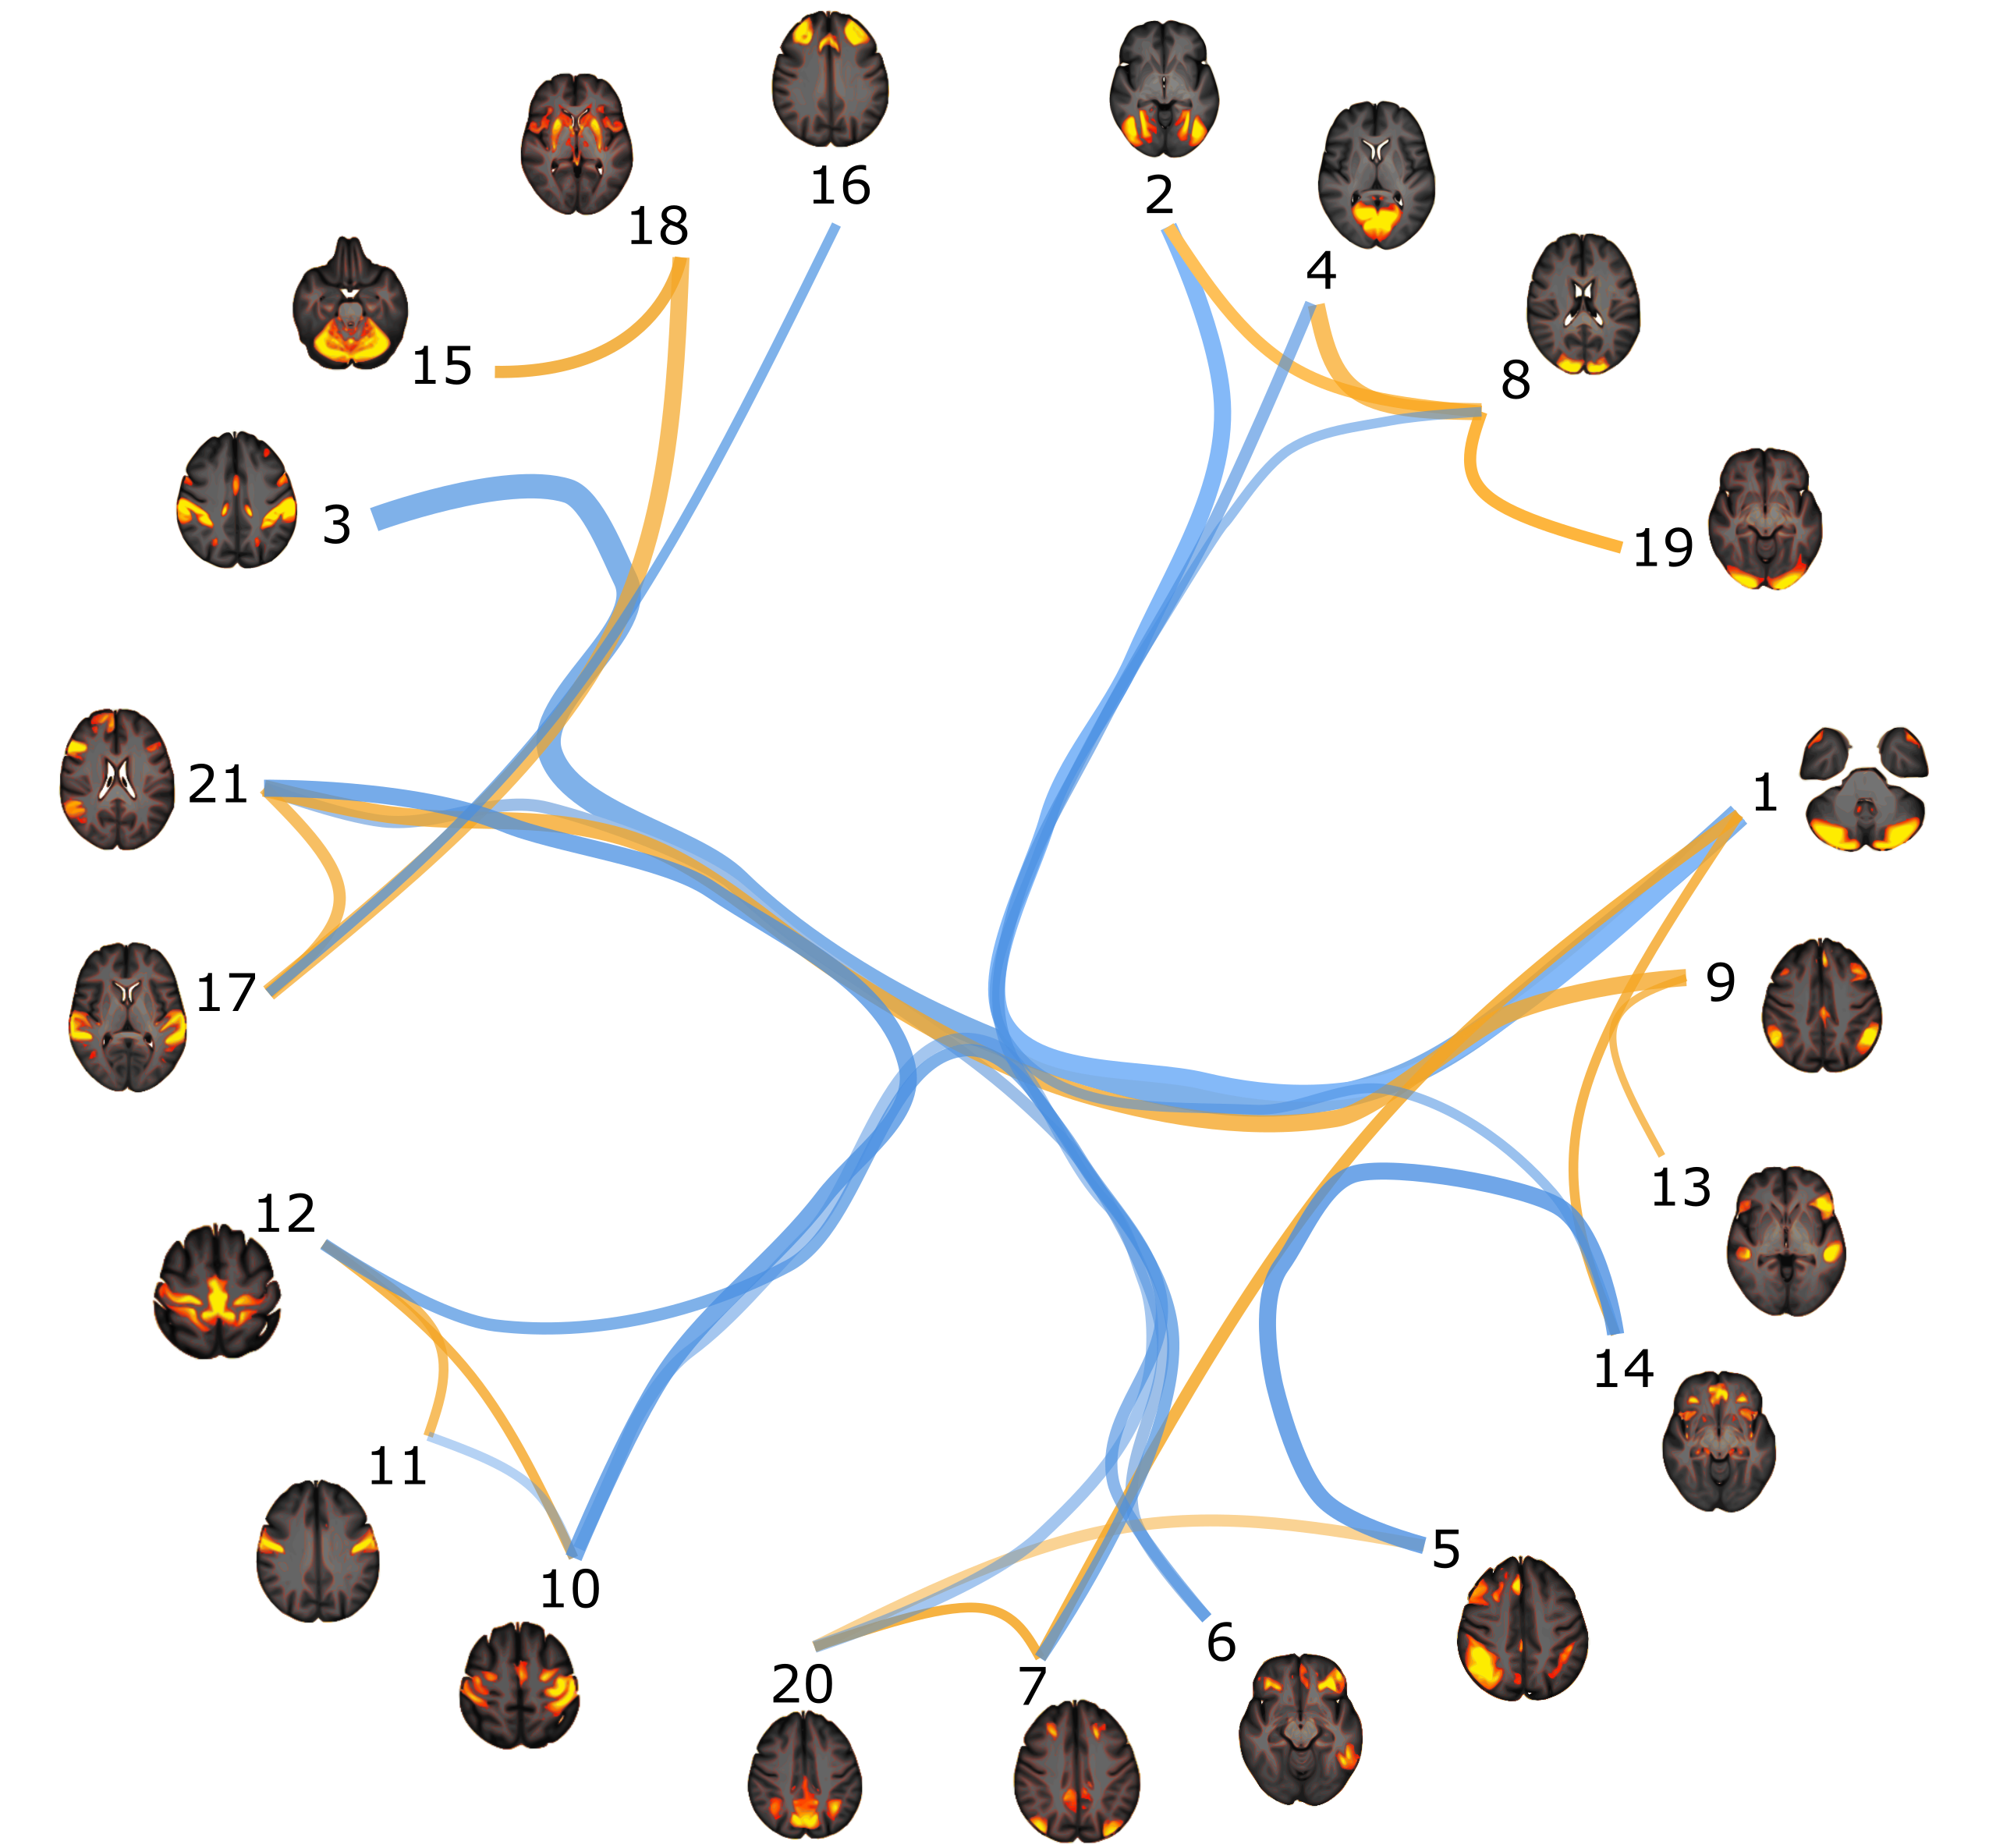
\includegraphics[width=0.6\textwidth]{chapters/images_methods/fmri_network_ukbiobank.png}
    \caption{A schematic visualisation of a network of functional brain networks. Blue and orange edges represent positive and negative correlation between brain networks, respectively.  The individual functional brain networks are represented as human brains with \acrshort{fmri} activations (orange), along the circumference of the circle. See \cref{tab:Networks} for the names of the functional brain networks. Image adapted from example at UK Biobank Brain Imaging Online Resources \cite{ukbiobank_brain_imaging}.}
    \label{fig:fmri_network}
\end{figure}

The graphs of functional brain networks used in this thesis are derived from \acrshort{fmri}. In short, functional \acrshort{mri} (\acrshort{fmri}) is a technique for measuring the neuronal activity in the human brain \cite{sporns}. In a measurement, the activations of various parts of the subject's brain are measured as time series. The correlations between these time series can then be calculated and formed into a network. Different sub-networks in the obtained \acrshort{fmri} brain network can often be associated with different functionalities of the brain. One example of such a functional brain network is the \acrfull{dmn}, which handles memory processing and mind wandering  \cite{alves_dmn}. The regions that make up the sub-networks do not necessarily have to be physically close together nor directly anatomically connected.

\todo{Byt färg på orange/blå i figuren om vi verkligen vill använda den här som atlas. Just nu okej, eftersom den bara är schematisk, men annars är den inkorrekt. }



\begin{table}[!htbp]
    \centering
    \caption{A key  of which node corresponds to what functional brain network in the data from the UK Biobank. See \cref{fig:fmri_network} for a representation of each functional brain network. Each node will in the remainder of this thesis be referred to by the abbreviation for its functional brain network.}
    \begin{tabular}{||c|c|c||}
        \hline
        Number & Network & Abbreviation  \\ \hline\hline
        1 & \acrlong{cb1} & \acrshort{cb1} \\ \hline
        2 & \acrlong{vl} & \acrshort{vl}  \\ \hline
        3 & \acrlong{ssn} & \acrshort{ssn} \\ \hline
        4 & \acrlong{vm} &  \acrshort{vm}\\ \hline
        5 & \acrlong{dar} & \acrshort{dar} \\ \hline
        6 & \acrlong{dal} &  \acrshort{dal} \\ \hline
        7 & \acrlong{fp} &  \acrshort{fp}\\ \hline
        8 & \acrlong{vv1m} & \acrshort{vv1m} \\ \hline
        9 & \acrlong{dmn} &  \acrshort{dmn} \\ \hline
        10 & \acrlong{pss} & \acrshort{pss} \\ \hline
        11 & \acrlong{pmn} & \acrshort{pmn} \\ \hline
        12 & \acrlong{smm} & \acrshort{smm}  \\ \hline
        13 & \acrlong{va} &  \acrshort{va}\\ \hline
        14 & \acrlong{sn} &  \acrshort{sn}\\ \hline
        15 & \acrlong{cb2} & \acrshort{cb2} \\ \hline
        16 & \acrlong{pl} & \acrshort{pl} \\ \hline
        17 & \acrlong{ts} & \acrshort{ts} \\ \hline
        18 & \acrlong{bg} &  \acrshort{bg} \\ \hline
        19 & \acrlong{vv1l} & \acrshort{vv1l} \\ \hline
        20 & \acrlong{pmc} & \acrshort{pmc} \\ \hline
        21 & \acrlong{tm} & \acrshort{tm} \\ \hline
    \end{tabular}
    \label{tab:Networks}
\end{table}


This thesis utilises \acrshort{fmri} data obtained form the UK Biobank for roughly 35000 subjects, of both sexes and varying between 45 and 80 years of age \cite{ukbiobank}. The \acrshort{fmri} data had been preprocessed and consisted of correlations between 21 different functional brain networks. The correlation between these 21 networks thus constituted a network of networks, and is interpreted as a graph where each node corresponds to one functional network and each edge the correlation between networks. A visualisation of such a brain graph is given in \cref{fig:fmri_network}, in which the various nodes and the functional brain networks they represent form the outer circle, with the coloured lines connecting the nodes being the edges in the graph. The lines are coloured according to the edge weights, with blue and orange lines having positive and negative weights respectively. For a list of what functional brain network each node corresponds to, and its abbreviation, see \cref{tab:Networks}.

\subsection{Handling negative edge weights}
A brain graph with both positive and negative weights may be problematic. Specifically, when normalising the adjacency matrices according to Equation \eqref{eq:renormalization_trick}, the risk of dividing by zero becomes imminent. There are several ways to handle this problem. One alternative is to only study all positive or all negative connections, and another might be to take the absolute value of all connections. We, however, decided to split the negative and positive connections into two separate graphs and thus form a multiplex graph. From a practical point of view this was implemented by creating a block diagonal adjacency matrix with all positive connections in the upper block and all negative connections in the lower block, see \cref{fig:block_diagonal_adjacency_matrix}. The connections in the positive block that were negative in the original adjacency matrix $A$ were replaced with zeros, and vice versa in the negative block.

\begin{figure}[!htbp]
    \centering
    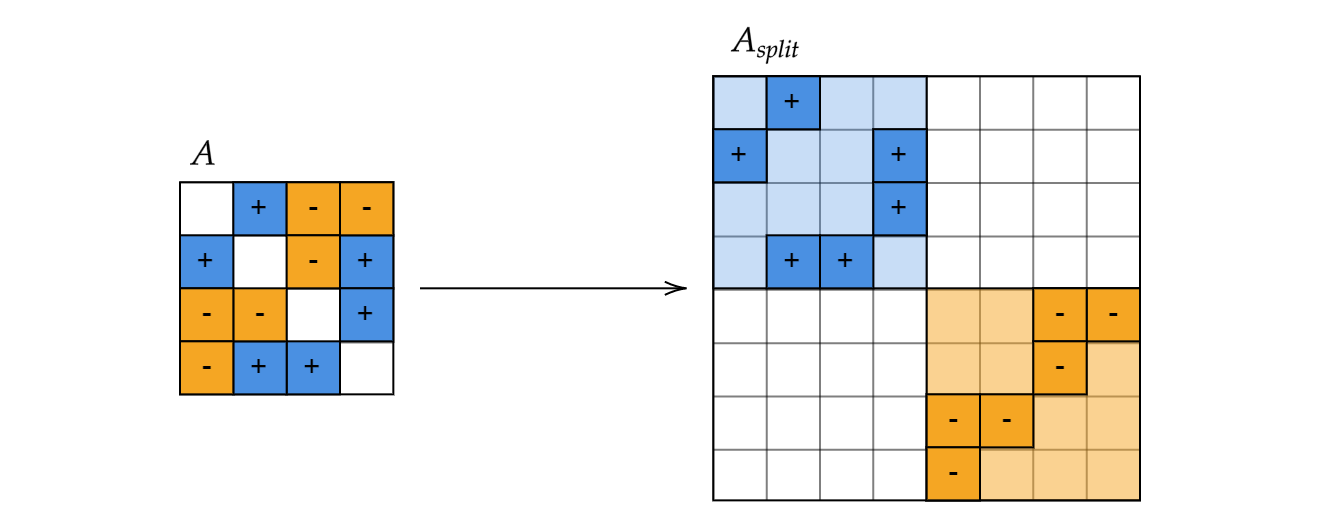
\includegraphics[width=0.9\textwidth]{chapters/images_methods/split.png}
    \caption{An example of how negative values in an adjacency matrix $A$ were handled. The negative values (orange) were extracted into the lower diagonal block of $A_{split}$, and replaced with zeros in the upper, positive block (blue).}
    \label{fig:block_diagonal_adjacency_matrix}
\end{figure}

\section{Models for graph classification}

Having described the preprocessing of the brain graphs, we now turn to the models used to perform graph prediction for individual subjects. Two models will be presented, a baseline regression model and a \acrshort{gcn} model, for the tasks of predicting subject age and sex.

\subsection{Baseline}
To validate how well the different \acrshort{gcn}-models performed, a baseline model had to be introduced for comparison. In this study, the baseline model consisted of a regression model where the connections between all of the nodes were regarded as separate input features. The adjacency matrix for an individual subject could then be viewed as a high dimensional data point, and the model thus aimed to fit a hyper plane to either separate the classes or predict a continuous variable. For a schematic view of the model see \cref{fig:Graph_class_baseline}. Note that the output layer has either two softmax-activated neurons in the case of sex classification or one neuron without activation in the case of age regression. 

From the definition of a graph in \cref{sec:general_graph_theory}, it follows that graphs are completely node order invariant, and several different ways of listing the connections results in the same graph. This might generally impose a problem since a regression model depend on its input being ordered. In this thesis, a regression model was, however, possible as a baseline model, since the brain graphs from the UK Biobank followed a consistent node ordering, and each input feature of the model was thus always the same connection. Furthermore, the regression model was also feasible due to the relatively small size of the brain graphs (21 nodes) compared to many other graphs (such as citation networks consisting of thousands of nodes). For larger graphs, models with one learnable parameter per connection would result in huge models. In that case, models that do not scale with the number of connections must be used, such as \acrshort{gcn}-based models. 

% \begin{center}
%     \resizebox {0.9\linewidth} {!} {
%         

\tikzset{every picture/.style={line width=0.75pt}} %set default line width to 0.75pt        

\begin{tikzpicture}[x=0.75pt,y=0.75pt,yscale=-1,xscale=1]
%uncomment if require: \path (0,256); %set diagram left start at 0, and has height of 256

%Straight Lines [id:da08012385894546048] 
\draw [color={rgb, 255:red, 0; green, 0; blue, 0 }  ,draw opacity=1 ]   (45,45) -- (185,130) ;
%Straight Lines [id:da8398961471148605] 
\draw [color={rgb, 255:red, 0; green, 0; blue, 0 }  ,draw opacity=1 ]   (45,85) -- (185,130) ;
%Straight Lines [id:da8832621988467466] 
\draw [color={rgb, 255:red, 0; green, 0; blue, 0 }  ,draw opacity=1 ]   (45,125) -- (185,130) ;
%Straight Lines [id:da8658449844223002] 
\draw [color={rgb, 255:red, 0; green, 0; blue, 0 }  ,draw opacity=1 ]   (45,215) -- (185,130) ;
%Straight Lines [id:da9842325204560114] 
\draw    (220,130) -- (270,130) ;
%Straight Lines [id:da9699253287015002] 
\draw    (280,110) -- (270,130) ;
%Straight Lines [id:da3136144075299854] 
\draw    (270,130) -- (280,150) ;
%Straight Lines [id:da4214591700017929] 
\draw    (280,110) -- (318,110) ;
\draw [shift={(320,110)}, rotate = 180] [fill={rgb, 255:red, 0; green, 0; blue, 0 }  ][line width=0.08]  [draw opacity=0] (12,-3) -- (0,0) -- (12,3) -- cycle    ;
%Straight Lines [id:da7746738186045765] 
\draw    (280,150) -- (318,150) ;
\draw [shift={(320,150)}, rotate = 180] [fill={rgb, 255:red, 0; green, 0; blue, 0 }  ][line width=0.08]  [draw opacity=0] (12,-3) -- (0,0) -- (12,3) -- cycle    ;
%Shape: Axis 2D [id:dp11393948673287424] 
\draw  (430,122.25) -- (460,122.25)(433,97.47) -- (433,125) (453,117.25) -- (460,122.25) -- (453,127.25) (428,104.47) -- (433,97.47) -- (438,104.47)  ;
%Straight Lines [id:da09576460905063744] 
\draw [color={rgb, 255:red, 74; green, 144; blue, 226 }  ,draw opacity=1 ]   (430,125) -- (451.67,103.33) -- (460,95) ;
%Shape: Axis 2D [id:dp12724162882260592] 
\draw  (430,157.07) -- (460,157.07)(433,135) -- (433,159.53) (453,152.07) -- (460,157.07) -- (453,162.07) (428,142) -- (433,135) -- (438,142)  ;
%Straight Lines [id:da9285983842245029] 
\draw [color={rgb, 255:red, 208; green, 2; blue, 27 }  ,draw opacity=1 ]   (440,137) -- (440,157) ;
%Straight Lines [id:da4541122584680737] 
\draw [color={rgb, 255:red, 74; green, 144; blue, 226 }  ,draw opacity=1 ]   (450,147) -- (450,157) ;

%Shape: Circle [id:dp5473399963870353] 
\draw  [fill={rgb, 255:red, 255; green, 255; blue, 255 }  ,fill opacity=1 ] (30,45) .. controls (30,36.72) and (36.72,30) .. (45,30) .. controls (53.28,30) and (60,36.72) .. (60,45) .. controls (60,53.28) and (53.28,60) .. (45,60) .. controls (36.72,60) and (30,53.28) .. (30,45) -- cycle ;
%Shape: Circle [id:dp9366596747620268] 
\draw  [fill={rgb, 255:red, 255; green, 255; blue, 255 }  ,fill opacity=1 ] (30,215) .. controls (30,206.72) and (36.72,200) .. (45,200) .. controls (53.28,200) and (60,206.72) .. (60,215) .. controls (60,223.28) and (53.28,230) .. (45,230) .. controls (36.72,230) and (30,223.28) .. (30,215) -- cycle ;
%Shape: Circle [id:dp6370056516541169] 
\draw  [fill={rgb, 255:red, 255; green, 255; blue, 255 }  ,fill opacity=1 ] (30,125) .. controls (30,116.72) and (36.72,110) .. (45,110) .. controls (53.28,110) and (60,116.72) .. (60,125) .. controls (60,133.28) and (53.28,140) .. (45,140) .. controls (36.72,140) and (30,133.28) .. (30,125) -- cycle ;
%Shape: Circle [id:dp6076795307057334] 
\draw  [fill={rgb, 255:red, 255; green, 255; blue, 255 }  ,fill opacity=1 ] (30,85) .. controls (30,76.72) and (36.72,70) .. (45,70) .. controls (53.28,70) and (60,76.72) .. (60,85) .. controls (60,93.28) and (53.28,100) .. (45,100) .. controls (36.72,100) and (30,93.28) .. (30,85) -- cycle ;
%Shape: Circle [id:dp15718416196861162] 
\draw  [fill={rgb, 255:red, 255; green, 255; blue, 255 }  ,fill opacity=1 ] (150,130) .. controls (150,110.67) and (165.67,95) .. (185,95) .. controls (204.33,95) and (220,110.67) .. (220,130) .. controls (220,149.33) and (204.33,165) .. (185,165) .. controls (165.67,165) and (150,149.33) .. (150,130) -- cycle ;

% Text Node
\draw (37,204.4) node [anchor=north west][inner sep=0.75pt]    {$x_{n}$};
% Text Node
\draw (37,114.4) node [anchor=north west][inner sep=0.75pt]    {$x_{3}$};
% Text Node
\draw (37,74.4) node [anchor=north west][inner sep=0.75pt]    {$x_{2}$};
% Text Node
\draw (37,34.4) node [anchor=north west][inner sep=0.75pt]    {$x_{1}$};
% Text Node
\draw (84,57.4) node [anchor=north west][inner sep=0.75pt]  [font=\scriptsize,color={rgb, 255:red, 0; green, 0; blue, 0 }  ,opacity=1 ]  {${\textstyle \theta _{1}}$};
% Text Node
\draw (84,87.4) node [anchor=north west][inner sep=0.75pt]  [font=\scriptsize,color={rgb, 255:red, 0; green, 0; blue, 0 }  ,opacity=1 ]  {${\textstyle \theta _{2}}$};
% Text Node
\draw (84,114.4) node [anchor=north west][inner sep=0.75pt]  [font=\scriptsize,color={rgb, 255:red, 0; green, 0; blue, 0 }  ,opacity=1 ]  {${\textstyle \theta _{3}}$};
% Text Node
\draw (84,157.4) node [anchor=north west][inner sep=0.75pt]  [font=\scriptsize,color={rgb, 255:red, 0; green, 0; blue, 0 }  ,opacity=1 ]  {${\textstyle \theta _{n}}$};
% Text Node
\draw (151,109.4) node [anchor=north west][inner sep=0.75pt]  [font=\footnotesize]  {$\sigma \left(\sum _{i} \theta _{i} x_{i}\right)$};
% Text Node
\draw (380,130) node   [align=left] {\begin{minipage}[lt]{68pt}\setlength\topsep{0pt}
\textbf{Age}
\begin{undefined}
\textit{or}
\end{undefined}
\textbf{Male/Female}
\end{minipage}};
% Text Node
\draw (241,109.4) node [anchor=north west][inner sep=0.75pt]    {$y$};
% Text Node
\draw (34,152.4) node [anchor=north west][inner sep=0.75pt]  [font=\Large]  {$\vdots $};


\end{tikzpicture}

%     }
% \end{center}

\begin{figure}[!htbp]
    \centering
    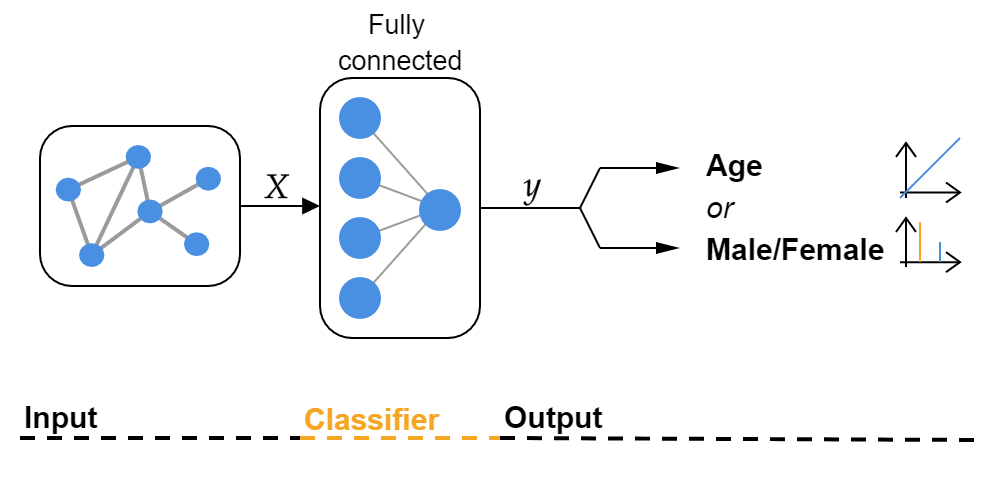
\includegraphics[width=0.7\textwidth]{chapters/images_methods/ffnn_v2.png}
    \caption{The baseline regression model. The adjacency matrix for a brain graph for a single subject forms the input, with a continuous value or class prediction as output in the case of age or sex prediction.}
    \label{fig:Graph_class_baseline}
\end{figure}

\subsection{GCN}

The motivation behind using \acrshort{gcn}-based models was that they hopefully would be able to extract information from the topological structure of the graphs, rather than simply studying the individual connections as, for instance, Baseline. A \acrshort{gcn}-based model, referred to simply as GCN, was thus developed. An illustration of the GCN model can be seen in \cref{fig:gcn_base}. GCN consisted of three consecutive graph convolutional layers, with propagation rule as defined in equation \eqref{eq:propagation_rule}, followed by a fully connected output layer. The graph convolutional layers had a \acrfull{relu} activation function and ten output features. This will be the case for all graph convolutional layers mentioned in the remainder of this thesis, unless otherwise specified. The input to the fully connected output layer consisted of the activations for all three graph convolutional layers, i.e. the activation for all feature maps in all layers, concatenated together. As described in \cref{sec:gcn} the activation of layer $i$ contains information about the $i$:th-order neighbourhood of each node. The inclusion of the activations after each layer in the classifier thus aimed to utilise information of how each node was embedded in a successively larger neighbourhood, which could be beneficial for the predictions.

The inputs to a graph convolutional model generally consists of an adjacency matrix $A$ and a node feature matrix $X$. However, the brain graphs in this thesis did not contain any information beyond connections that could be associated with specific nodes. GCN thus used a \textit{featureless} approach, in which the feature matrix was taken to be the identity matrix, $X=I$ \cite{kipf_vae}.

% \begin{center}
%     \resizebox {0.9\linewidth} {!} {
%         

\tikzset{every picture/.style={line width=0.75pt}} %set default line width to 0.75pt        

\begin{tikzpicture}[x=0.75pt,y=0.75pt,yscale=-1,xscale=1]
%uncomment if require: \path (0,268); %set diagram left start at 0, and has height of 268

%Rounded Rect [id:dp1454512597044859] 
\draw  [fill={rgb, 255:red, 255; green, 255; blue, 255 }  ,fill opacity=1 ] (150,48) .. controls (150,38.06) and (158.06,30) .. (168,30) -- (222,30) .. controls (231.94,30) and (240,38.06) .. (240,48) -- (240,222) .. controls (240,231.94) and (231.94,240) .. (222,240) -- (168,240) .. controls (158.06,240) and (150,231.94) .. (150,222) -- cycle ;
%Straight Lines [id:da44371133423221676] 
\draw [color={rgb, 255:red, 155; green, 155; blue, 155 }  ,draw opacity=1 ][line width=1.5]    (169.29,109.19) -- (177.86,134.65) ;
%Straight Lines [id:da3398362409006068] 
\draw [color={rgb, 255:red, 155; green, 155; blue, 155 }  ,draw opacity=1 ][line width=1.5]    (169.29,109.19) -- (195,96.46) ;
%Shape: Ellipse [id:dp7222477940626566] 
\draw  [color={rgb, 255:red, 245; green, 166; blue, 35 }  ,draw opacity=1 ][fill={rgb, 255:red, 245; green, 166; blue, 35 }  ,fill opacity=1 ] (165,109.19) .. controls (165,106.85) and (166.92,104.95) .. (169.29,104.95) .. controls (171.65,104.95) and (173.57,106.85) .. (173.57,109.19) .. controls (173.57,111.53) and (171.65,113.43) .. (169.29,113.43) .. controls (166.92,113.43) and (165,111.53) .. (165,109.19) -- cycle ;
%Straight Lines [id:da7434143201874741] 
\draw [color={rgb, 255:red, 155; green, 155; blue, 155 }  ,draw opacity=1 ][line width=1.5]    (199.29,63.23) -- (195,42.02) ;
%Straight Lines [id:da17541088644592207] 
\draw [color={rgb, 255:red, 155; green, 155; blue, 155 }  ,draw opacity=0.4 ][line width=1.5]    (177.86,80.2) -- (195,42.02) ;
%Straight Lines [id:da49554490131335505] 
\draw [color={rgb, 255:red, 155; green, 155; blue, 155 }  ,draw opacity=0.4 ][line width=1.5]    (169.29,54.75) -- (177.86,80.2) ;
%Straight Lines [id:da7823220018723711] 
\draw [color={rgb, 255:red, 155; green, 155; blue, 155 }  ,draw opacity=1 ][line width=1.5]    (199.29,63.23) -- (220.71,50.51) ;
%Straight Lines [id:da4144720186472177] 
\draw [color={rgb, 255:red, 155; green, 155; blue, 155 }  ,draw opacity=0.4 ][fill={rgb, 255:red, 0; green, 0; blue, 0 }  ,fill opacity=0.5 ][line width=1.5]    (169.29,54.75) -- (195,42.02) ;
%Straight Lines [id:da4512038117618906] 
\draw [color={rgb, 255:red, 155; green, 155; blue, 155 }  ,draw opacity=1 ][line width=1.5]    (199.29,63.23) -- (177.86,80.2) ;
%Straight Lines [id:da6717586155874848] 
\draw [color={rgb, 255:red, 155; green, 155; blue, 155 }  ,draw opacity=1 ][line width=1.5]    (199.29,63.23) -- (216.43,75.96) ;
%Shape: Ellipse [id:dp8214542913209517] 
\draw  [color={rgb, 255:red, 167; green, 207; blue, 255 }  ,draw opacity=1 ][fill={rgb, 255:red, 167; green, 207; blue, 255 }  ,fill opacity=1 ] (165,54.75) .. controls (165,52.4) and (166.92,50.51) .. (169.29,50.51) .. controls (171.65,50.51) and (173.57,52.4) .. (173.57,54.75) .. controls (173.57,57.09) and (171.65,58.99) .. (169.29,58.99) .. controls (166.92,58.99) and (165,57.09) .. (165,54.75) -- cycle ;
%Shape: Ellipse [id:dp47038889017471486] 
\draw  [color={rgb, 255:red, 74; green, 144; blue, 226 }  ,draw opacity=1 ][fill={rgb, 255:red, 74; green, 144; blue, 226 }  ,fill opacity=1 ] (173.57,80.2) .. controls (173.57,77.86) and (175.49,75.96) .. (177.86,75.96) .. controls (180.22,75.96) and (182.14,77.86) .. (182.14,80.2) .. controls (182.14,82.55) and (180.22,84.44) .. (177.86,84.44) .. controls (175.49,84.44) and (173.57,82.55) .. (173.57,80.2) -- cycle ;
%Shape: Ellipse [id:dp10306056601214997] 
\draw  [color={rgb, 255:red, 245; green, 166; blue, 35 }  ,draw opacity=1 ][fill={rgb, 255:red, 245; green, 166; blue, 35 }  ,fill opacity=1 ] (195,63.23) .. controls (195,60.89) and (196.92,58.99) .. (199.29,58.99) .. controls (201.65,58.99) and (203.57,60.89) .. (203.57,63.23) .. controls (203.57,65.58) and (201.65,67.47) .. (199.29,67.47) .. controls (196.92,67.47) and (195,65.58) .. (195,63.23) -- cycle ;
%Shape: Ellipse [id:dp3356200716848863] 
\draw  [color={rgb, 255:red, 74; green, 144; blue, 226 }  ,draw opacity=1 ][fill={rgb, 255:red, 74; green, 144; blue, 226 }  ,fill opacity=1 ] (212.14,75.96) .. controls (212.14,73.62) and (214.06,71.72) .. (216.43,71.72) .. controls (218.8,71.72) and (220.71,73.62) .. (220.71,75.96) .. controls (220.71,78.3) and (218.8,80.2) .. (216.43,80.2) .. controls (214.06,80.2) and (212.14,78.3) .. (212.14,75.96) -- cycle ;
%Shape: Ellipse [id:dp9107615531803757] 
\draw  [color={rgb, 255:red, 74; green, 144; blue, 226 }  ,draw opacity=1 ][fill={rgb, 255:red, 74; green, 144; blue, 226 }  ,fill opacity=1 ] (190.71,42.02) .. controls (190.71,39.68) and (192.63,37.78) .. (195,37.78) .. controls (197.37,37.78) and (199.29,39.68) .. (199.29,42.02) .. controls (199.29,44.36) and (197.37,46.26) .. (195,46.26) .. controls (192.63,46.26) and (190.71,44.36) .. (190.71,42.02) -- cycle ;
%Shape: Ellipse [id:dp686194905732459] 
\draw  [color={rgb, 255:red, 74; green, 144; blue, 226 }  ,draw opacity=1 ][fill={rgb, 255:red, 74; green, 144; blue, 226 }  ,fill opacity=1 ] (216.43,50.51) .. controls (216.43,48.16) and (218.35,46.26) .. (220.71,46.26) .. controls (223.08,46.26) and (225,48.16) .. (225,50.51) .. controls (225,52.85) and (223.08,54.75) .. (220.71,54.75) .. controls (218.35,54.75) and (216.43,52.85) .. (216.43,50.51) -- cycle ;
%Straight Lines [id:da4462253100757778] 
\draw [color={rgb, 255:red, 155; green, 155; blue, 155 }  ,draw opacity=1 ][line width=1.5]    (177.86,227.98) -- (195,189.8) ;
%Straight Lines [id:da33046752635028676] 
\draw [color={rgb, 255:red, 155; green, 155; blue, 155 }  ,draw opacity=1 ][line width=1.5]    (169.29,202.53) -- (177.86,227.98) ;
%Straight Lines [id:da45388559372006365] 
\draw [color={rgb, 255:red, 155; green, 155; blue, 155 }  ,draw opacity=1 ][line width=1.5]    (199.29,211.01) -- (177.86,227.98) ;
%Shape: Ellipse [id:dp12334564292514116] 
\draw  [color={rgb, 255:red, 245; green, 166; blue, 35 }  ,draw opacity=1 ][fill={rgb, 255:red, 245; green, 166; blue, 35 }  ,fill opacity=1 ] (173.57,227.98) .. controls (173.57,225.64) and (175.49,223.74) .. (177.86,223.74) .. controls (180.22,223.74) and (182.14,225.64) .. (182.14,227.98) .. controls (182.14,230.32) and (180.22,232.22) .. (177.86,232.22) .. controls (175.49,232.22) and (173.57,230.32) .. (173.57,227.98) -- cycle ;
%Straight Lines [id:da5879944549609841] 
\draw [color={rgb, 255:red, 155; green, 155; blue, 155 }  ,draw opacity=0.4 ][fill={rgb, 255:red, 0; green, 0; blue, 0 }  ,fill opacity=0.5 ][line width=1.5]    (195,96.46) -- (177.86,134.65) ;
%Straight Lines [id:da10478801456064013] 
\draw [color={rgb, 255:red, 155; green, 155; blue, 155 }  ,draw opacity=0.4 ][fill={rgb, 255:red, 0; green, 0; blue, 0 }  ,fill opacity=0.5 ][line width=1.5]    (195,96.46) -- (199.29,117.68) ;
%Straight Lines [id:da5465003287874521] 
\draw [color={rgb, 255:red, 155; green, 155; blue, 155 }  ,draw opacity=0.4 ][fill={rgb, 255:red, 0; green, 0; blue, 0 }  ,fill opacity=0.5 ][line width=1.5]    (177.86,134.65) -- (199.29,117.68) ;
%Straight Lines [id:da029197166814233233] 
\draw [color={rgb, 255:red, 155; green, 155; blue, 155 }  ,draw opacity=0.4 ][fill={rgb, 255:red, 0; green, 0; blue, 0 }  ,fill opacity=0.5 ][line width=1.5]    (199.29,117.68) -- (220.71,104.95) ;
%Straight Lines [id:da7886430348639939] 
\draw [color={rgb, 255:red, 155; green, 155; blue, 155 }  ,draw opacity=0.4 ][fill={rgb, 255:red, 0; green, 0; blue, 0 }  ,fill opacity=0.5 ][line width=1.5]    (199.29,117.68) -- (216.43,130.4) ;
%Straight Lines [id:da48838206548505325] 
\draw [color={rgb, 255:red, 155; green, 155; blue, 155 }  ,draw opacity=0.4 ][fill={rgb, 255:red, 0; green, 0; blue, 0 }  ,fill opacity=0.5 ][line width=1.5]    (195,189.8) -- (169.29,202.53) ;
%Straight Lines [id:da6023020962352053] 
\draw [color={rgb, 255:red, 155; green, 155; blue, 155 }  ,draw opacity=0.4 ][fill={rgb, 255:red, 0; green, 0; blue, 0 }  ,fill opacity=0.5 ][line width=1.5]    (195,189.8) -- (199.29,211.01) ;
%Straight Lines [id:da9783904688690421] 
\draw [color={rgb, 255:red, 155; green, 155; blue, 155 }  ,draw opacity=0.4 ][fill={rgb, 255:red, 0; green, 0; blue, 0 }  ,fill opacity=0.5 ][line width=1.5]    (220.71,198.28) -- (199.29,211.01) ;
%Shape: Ellipse [id:dp3754045964979047] 
\draw  [color={rgb, 255:red, 74; green, 144; blue, 226 }  ,draw opacity=1 ][fill={rgb, 255:red, 74; green, 144; blue, 226 }  ,fill opacity=1 ] (190.71,189.8) .. controls (190.71,187.45) and (192.63,185.56) .. (195,185.56) .. controls (197.37,185.56) and (199.29,187.45) .. (199.29,189.8) .. controls (199.29,192.14) and (197.37,194.04) .. (195,194.04) .. controls (192.63,194.04) and (190.71,192.14) .. (190.71,189.8) -- cycle ;
%Shape: Ellipse [id:dp64113309900183] 
\draw  [color={rgb, 255:red, 167; green, 207; blue, 255 }  ,draw opacity=1 ][fill={rgb, 255:red, 167; green, 207; blue, 255 }  ,fill opacity=1 ] (216.43,198.28) .. controls (216.43,195.94) and (218.35,194.04) .. (220.71,194.04) .. controls (223.08,194.04) and (225,195.94) .. (225,198.28) .. controls (225,200.63) and (223.08,202.53) .. (220.71,202.53) .. controls (218.35,202.53) and (216.43,200.63) .. (216.43,198.28) -- cycle ;
%Shape: Ellipse [id:dp691449696768264] 
\draw  [color={rgb, 255:red, 74; green, 144; blue, 226 }  ,draw opacity=1 ][fill={rgb, 255:red, 74; green, 144; blue, 226 }  ,fill opacity=1 ] (165,202.53) .. controls (165,200.18) and (166.92,198.28) .. (169.29,198.28) .. controls (171.65,198.28) and (173.57,200.18) .. (173.57,202.53) .. controls (173.57,204.87) and (171.65,206.77) .. (169.29,206.77) .. controls (166.92,206.77) and (165,204.87) .. (165,202.53) -- cycle ;
%Straight Lines [id:da03064657141642635] 
\draw [color={rgb, 255:red, 155; green, 155; blue, 155 }  ,draw opacity=0.4 ][fill={rgb, 255:red, 0; green, 0; blue, 0 }  ,fill opacity=0.5 ][line width=1.5]    (216.43,223.74) -- (199.29,211.01) ;
%Shape: Ellipse [id:dp07058389708117052] 
\draw  [color={rgb, 255:red, 74; green, 144; blue, 226 }  ,draw opacity=1 ][fill={rgb, 255:red, 74; green, 144; blue, 226 }  ,fill opacity=1 ] (195,211.01) .. controls (195,208.67) and (196.92,206.77) .. (199.29,206.77) .. controls (201.65,206.77) and (203.57,208.67) .. (203.57,211.01) .. controls (203.57,213.35) and (201.65,215.25) .. (199.29,215.25) .. controls (196.92,215.25) and (195,213.35) .. (195,211.01) -- cycle ;
%Shape: Ellipse [id:dp697421628639054] 
\draw  [color={rgb, 255:red, 167; green, 207; blue, 255 }  ,draw opacity=1 ][fill={rgb, 255:red, 167; green, 207; blue, 255 }  ,fill opacity=1 ] (212.14,223.74) .. controls (212.14,221.39) and (214.06,219.49) .. (216.43,219.49) .. controls (218.8,219.49) and (220.71,221.39) .. (220.71,223.74) .. controls (220.71,226.08) and (218.8,227.98) .. (216.43,227.98) .. controls (214.06,227.98) and (212.14,226.08) .. (212.14,223.74) -- cycle ;
%Shape: Ellipse [id:dp8717393277655574] 
\draw  [color={rgb, 255:red, 167; green, 207; blue, 255 }  ,draw opacity=1 ][fill={rgb, 255:red, 167; green, 207; blue, 255 }  ,fill opacity=1 ] (195,117.68) .. controls (195,115.33) and (196.92,113.43) .. (199.29,113.43) .. controls (201.65,113.43) and (203.57,115.33) .. (203.57,117.68) .. controls (203.57,120.02) and (201.65,121.92) .. (199.29,121.92) .. controls (196.92,121.92) and (195,120.02) .. (195,117.68) -- cycle ;
%Shape: Ellipse [id:dp770793755049425] 
\draw  [color={rgb, 255:red, 167; green, 207; blue, 255 }  ,draw opacity=1 ][fill={rgb, 255:red, 167; green, 207; blue, 255 }  ,fill opacity=1 ] (212.14,130.4) .. controls (212.14,128.06) and (214.06,126.16) .. (216.43,126.16) .. controls (218.8,126.16) and (220.71,128.06) .. (220.71,130.4) .. controls (220.71,132.75) and (218.8,134.65) .. (216.43,134.65) .. controls (214.06,134.65) and (212.14,132.75) .. (212.14,130.4) -- cycle ;
%Shape: Ellipse [id:dp6425563981873512] 
\draw  [color={rgb, 255:red, 167; green, 207; blue, 255 }  ,draw opacity=1 ][fill={rgb, 255:red, 167; green, 207; blue, 255 }  ,fill opacity=1 ] (216.43,104.95) .. controls (216.43,102.61) and (218.35,100.71) .. (220.71,100.71) .. controls (223.08,100.71) and (225,102.61) .. (225,104.95) .. controls (225,107.29) and (223.08,109.19) .. (220.71,109.19) .. controls (218.35,109.19) and (216.43,107.29) .. (216.43,104.95) -- cycle ;
%Shape: Ellipse [id:dp6740261081738981] 
\draw  [color={rgb, 255:red, 74; green, 144; blue, 226 }  ,draw opacity=1 ][fill={rgb, 255:red, 74; green, 144; blue, 226 }  ,fill opacity=1 ] (190.71,96.46) .. controls (190.71,94.12) and (192.63,92.22) .. (195,92.22) .. controls (197.37,92.22) and (199.29,94.12) .. (199.29,96.46) .. controls (199.29,98.81) and (197.37,100.71) .. (195,100.71) .. controls (192.63,100.71) and (190.71,98.81) .. (190.71,96.46) -- cycle ;
%Shape: Ellipse [id:dp04602563531483872] 
\draw  [color={rgb, 255:red, 74; green, 144; blue, 226 }  ,draw opacity=1 ][fill={rgb, 255:red, 74; green, 144; blue, 226 }  ,fill opacity=1 ] (173.57,134.65) .. controls (173.57,132.3) and (175.49,130.4) .. (177.86,130.4) .. controls (180.22,130.4) and (182.14,132.3) .. (182.14,134.65) .. controls (182.14,136.99) and (180.22,138.89) .. (177.86,138.89) .. controls (175.49,138.89) and (173.57,136.99) .. (173.57,134.65) -- cycle ;
%Shape: Ellipse [id:dp7012237407172539] 
\draw  [fill={rgb, 255:red, 0; green, 0; blue, 0 }  ,fill opacity=1 ] (193.5,159.89) .. controls (193.5,158.6) and (194.51,157.56) .. (195.75,157.56) .. controls (196.99,157.56) and (198,158.6) .. (198,159.89) .. controls (198,161.18) and (196.99,162.22) .. (195.75,162.22) .. controls (194.51,162.22) and (193.5,161.18) .. (193.5,159.89) -- cycle ;
%Shape: Ellipse [id:dp3114230595274974] 
\draw  [fill={rgb, 255:red, 0; green, 0; blue, 0 }  ,fill opacity=1 ] (193.5,150.56) .. controls (193.5,149.27) and (194.51,148.22) .. (195.75,148.22) .. controls (196.99,148.22) and (198,149.27) .. (198,150.56) .. controls (198,151.84) and (196.99,152.89) .. (195.75,152.89) .. controls (194.51,152.89) and (193.5,151.84) .. (193.5,150.56) -- cycle ;
%Shape: Ellipse [id:dp37386234270345065] 
\draw  [fill={rgb, 255:red, 0; green, 0; blue, 0 }  ,fill opacity=1 ] (193.5,169.22) .. controls (193.5,167.93) and (194.51,166.89) .. (195.75,166.89) .. controls (196.99,166.89) and (198,167.93) .. (198,169.22) .. controls (198,170.51) and (196.99,171.56) .. (195.75,171.56) .. controls (194.51,171.56) and (193.5,170.51) .. (193.5,169.22) -- cycle ;

%Rounded Rect [id:dp9087802921841164] 
\draw   (260,128) .. controls (260,123.58) and (263.58,120) .. (268,120) -- (302,120) .. controls (306.42,120) and (310,123.58) .. (310,128) -- (310,152) .. controls (310,156.42) and (306.42,160) .. (302,160) -- (268,160) .. controls (263.58,160) and (260,156.42) .. (260,152) -- cycle ;
%Straight Lines [id:da04447467340422939] 
\draw    (310,140) -- (330,140) ;
%Straight Lines [id:da5334327028246098] 
\draw [color={rgb, 255:red, 155; green, 155; blue, 155 }  ,draw opacity=1 ][line width=1.5]    (65.01,142.73) -- (59.17,115.45) ;
%Straight Lines [id:da4099968368068212] 
\draw [color={rgb, 255:red, 155; green, 155; blue, 155 }  ,draw opacity=1 ][line width=1.5]    (35.85,164.55) -- (59.17,115.45) ;
%Straight Lines [id:da8075613001249213] 
\draw [color={rgb, 255:red, 155; green, 155; blue, 155 }  ,draw opacity=1 ][line width=1.5]    (24.18,131.82) -- (35.85,164.55) ;
%Straight Lines [id:da7949764047700321] 
\draw [color={rgb, 255:red, 155; green, 155; blue, 155 }  ,draw opacity=1 ][line width=1.5]    (65.01,142.73) -- (94.17,126.36) ;
%Straight Lines [id:da4886477553077586] 
\draw [color={rgb, 255:red, 155; green, 155; blue, 155 }  ,draw opacity=1 ][line width=1.5]    (24.18,131.82) -- (59.17,115.45) ;
%Straight Lines [id:da4437033864911011] 
\draw [color={rgb, 255:red, 155; green, 155; blue, 155 }  ,draw opacity=1 ][line width=1.5]    (65.01,142.73) -- (35.85,164.55) ;
%Straight Lines [id:da6182912079509322] 
\draw [color={rgb, 255:red, 155; green, 155; blue, 155 }  ,draw opacity=1 ][line width=1.5]    (65.01,142.73) -- (88.34,159.09) ;
%Shape: Ellipse [id:dp11646472758372184] 
\draw  [color={rgb, 255:red, 74; green, 144; blue, 226 }  ,draw opacity=1 ][fill={rgb, 255:red, 74; green, 144; blue, 226 }  ,fill opacity=1 ] (18.35,131.82) .. controls (18.35,128.81) and (20.96,126.36) .. (24.18,126.36) .. controls (27.4,126.36) and (30.01,128.81) .. (30.01,131.82) .. controls (30.01,134.83) and (27.4,137.27) .. (24.18,137.27) .. controls (20.96,137.27) and (18.35,134.83) .. (18.35,131.82) -- cycle ;
%Shape: Ellipse [id:dp0497507523482601] 
\draw  [color={rgb, 255:red, 74; green, 144; blue, 226 }  ,draw opacity=1 ][fill={rgb, 255:red, 74; green, 144; blue, 226 }  ,fill opacity=1 ] (30.01,164.55) .. controls (30.01,161.53) and (32.63,159.09) .. (35.85,159.09) .. controls (39.07,159.09) and (41.68,161.53) .. (41.68,164.55) .. controls (41.68,167.56) and (39.07,170) .. (35.85,170) .. controls (32.63,170) and (30.01,167.56) .. (30.01,164.55) -- cycle ;
%Shape: Ellipse [id:dp923504470392968] 
\draw  [color={rgb, 255:red, 74; green, 144; blue, 226 }  ,draw opacity=1 ][fill={rgb, 255:red, 74; green, 144; blue, 226 }  ,fill opacity=1 ] (59.17,142.73) .. controls (59.17,139.71) and (61.79,137.27) .. (65.01,137.27) .. controls (68.23,137.27) and (70.84,139.71) .. (70.84,142.73) .. controls (70.84,145.74) and (68.23,148.18) .. (65.01,148.18) .. controls (61.79,148.18) and (59.17,145.74) .. (59.17,142.73) -- cycle ;
%Shape: Ellipse [id:dp44760031358442776] 
\draw  [color={rgb, 255:red, 74; green, 144; blue, 226 }  ,draw opacity=1 ][fill={rgb, 255:red, 74; green, 144; blue, 226 }  ,fill opacity=1 ] (82.5,159.09) .. controls (82.5,156.08) and (85.11,153.64) .. (88.34,153.64) .. controls (91.56,153.64) and (94.17,156.08) .. (94.17,159.09) .. controls (94.17,162.1) and (91.56,164.55) .. (88.34,164.55) .. controls (85.11,164.55) and (82.5,162.1) .. (82.5,159.09) -- cycle ;
%Shape: Ellipse [id:dp0773933591251863] 
\draw  [color={rgb, 255:red, 74; green, 144; blue, 226 }  ,draw opacity=1 ][fill={rgb, 255:red, 74; green, 144; blue, 226 }  ,fill opacity=1 ] (53.34,115.45) .. controls (53.34,112.44) and (55.95,110) .. (59.17,110) .. controls (62.4,110) and (65.01,112.44) .. (65.01,115.45) .. controls (65.01,118.47) and (62.4,120.91) .. (59.17,120.91) .. controls (55.95,120.91) and (53.34,118.47) .. (53.34,115.45) -- cycle ;
%Shape: Ellipse [id:dp4981680059611522] 
\draw  [color={rgb, 255:red, 74; green, 144; blue, 226 }  ,draw opacity=1 ][fill={rgb, 255:red, 74; green, 144; blue, 226 }  ,fill opacity=1 ] (88.34,126.36) .. controls (88.34,123.35) and (90.95,120.91) .. (94.17,120.91) .. controls (97.39,120.91) and (100,123.35) .. (100,126.36) .. controls (100,129.38) and (97.39,131.82) .. (94.17,131.82) .. controls (90.95,131.82) and (88.34,129.38) .. (88.34,126.36) -- cycle ;

%Rounded Rect [id:dp855215770961127] 
\draw   (10,116) .. controls (10,107.16) and (17.16,100) .. (26,100) -- (94,100) .. controls (102.84,100) and (110,107.16) .. (110,116) -- (110,164) .. controls (110,172.84) and (102.84,180) .. (94,180) -- (26,180) .. controls (17.16,180) and (10,172.84) .. (10,164) -- cycle ;
%Straight Lines [id:da865822603980609] 
\draw    (110,140) -- (150,140) ;
%Straight Lines [id:da4781293941355824] 
\draw    (420,140) -- (470,140) ;
%Straight Lines [id:da9997190507560019] 
\draw    (480,120) -- (470,140) ;
%Straight Lines [id:da9897698727052839] 
\draw    (470,140) -- (480,160) ;
%Straight Lines [id:da5250020646100277] 
\draw    (480,120) -- (518,120) ;
\draw [shift={(520,120)}, rotate = 180] [fill={rgb, 255:red, 0; green, 0; blue, 0 }  ][line width=0.08]  [draw opacity=0] (12,-3) -- (0,0) -- (12,3) -- cycle    ;
%Straight Lines [id:da8007130287528326] 
\draw    (480,160) -- (518,160) ;
\draw [shift={(520,160)}, rotate = 180] [fill={rgb, 255:red, 0; green, 0; blue, 0 }  ][line width=0.08]  [draw opacity=0] (12,-3) -- (0,0) -- (12,3) -- cycle    ;
%Shape: Axis 2D [id:dp12898164037662085] 
\draw  (630,132.25) -- (660,132.25)(633,107.47) -- (633,135) (653,127.25) -- (660,132.25) -- (653,137.25) (628,114.47) -- (633,107.47) -- (638,114.47)  ;
%Straight Lines [id:da8546091575274994] 
\draw [color={rgb, 255:red, 74; green, 144; blue, 226 }  ,draw opacity=1 ]   (630,135) -- (651.67,113.33) -- (660,105) ;
%Shape: Axis 2D [id:dp3159900508610336] 
\draw  (630,167.07) -- (660,167.07)(633,145) -- (633,169.53) (653,162.07) -- (660,167.07) -- (653,172.07) (628,152) -- (633,145) -- (638,152)  ;
%Straight Lines [id:da2214390871002745] 
\draw [color={rgb, 255:red, 208; green, 2; blue, 27 }  ,draw opacity=1 ]   (640,147) -- (640,167) ;
%Straight Lines [id:da5235485948286522] 
\draw [color={rgb, 255:red, 74; green, 144; blue, 226 }  ,draw opacity=1 ]   (650,157) -- (650,167) ;

%Straight Lines [id:da0011855880200477564] 
\draw    (240,140) -- (260,140) ;
%Rounded Rect [id:dp3640479469957574] 
\draw  [fill={rgb, 255:red, 255; green, 255; blue, 255 }  ,fill opacity=1 ] (330,48) .. controls (330,38.06) and (338.06,30) .. (348,30) -- (402,30) .. controls (411.94,30) and (420,38.06) .. (420,48) -- (420,222) .. controls (420,231.94) and (411.94,240) .. (402,240) -- (348,240) .. controls (338.06,240) and (330,231.94) .. (330,222) -- cycle ;
%Straight Lines [id:da36833369698003215] 
\draw [color={rgb, 255:red, 155; green, 155; blue, 155 }  ,draw opacity=1 ][line width=1.5]    (349.29,109.19) -- (357.86,134.65) ;
%Straight Lines [id:da7140367877186562] 
\draw [color={rgb, 255:red, 155; green, 155; blue, 155 }  ,draw opacity=1 ][line width=1.5]    (349.29,109.19) -- (375,96.46) ;
%Shape: Ellipse [id:dp30211957071106843] 
\draw  [color={rgb, 255:red, 245; green, 166; blue, 35 }  ,draw opacity=1 ][fill={rgb, 255:red, 245; green, 166; blue, 35 }  ,fill opacity=1 ] (345,109.19) .. controls (345,106.85) and (346.92,104.95) .. (349.29,104.95) .. controls (351.65,104.95) and (353.57,106.85) .. (353.57,109.19) .. controls (353.57,111.53) and (351.65,113.43) .. (349.29,113.43) .. controls (346.92,113.43) and (345,111.53) .. (345,109.19) -- cycle ;
%Straight Lines [id:da17408965111455865] 
\draw [color={rgb, 255:red, 155; green, 155; blue, 155 }  ,draw opacity=1 ][line width=1.5]    (379.29,63.23) -- (375,42.02) ;
%Straight Lines [id:da08473532854907884] 
\draw [color={rgb, 255:red, 155; green, 155; blue, 155 }  ,draw opacity=0.4 ][line width=1.5]    (357.86,80.2) -- (375,42.02) ;
%Straight Lines [id:da5880812032491216] 
\draw [color={rgb, 255:red, 155; green, 155; blue, 155 }  ,draw opacity=0.4 ][line width=1.5]    (349.29,54.75) -- (357.86,80.2) ;
%Straight Lines [id:da9621297667966422] 
\draw [color={rgb, 255:red, 155; green, 155; blue, 155 }  ,draw opacity=1 ][line width=1.5]    (379.29,63.23) -- (400.71,50.51) ;
%Straight Lines [id:da6752975937599959] 
\draw [color={rgb, 255:red, 155; green, 155; blue, 155 }  ,draw opacity=0.4 ][fill={rgb, 255:red, 0; green, 0; blue, 0 }  ,fill opacity=0.5 ][line width=1.5]    (349.29,54.75) -- (375,42.02) ;
%Straight Lines [id:da09574905139243506] 
\draw [color={rgb, 255:red, 155; green, 155; blue, 155 }  ,draw opacity=1 ][line width=1.5]    (379.29,63.23) -- (357.86,80.2) ;
%Straight Lines [id:da010518874424237268] 
\draw [color={rgb, 255:red, 155; green, 155; blue, 155 }  ,draw opacity=1 ][line width=1.5]    (379.29,63.23) -- (396.43,75.96) ;
%Shape: Ellipse [id:dp8663719631601869] 
\draw  [color={rgb, 255:red, 167; green, 207; blue, 255 }  ,draw opacity=1 ][fill={rgb, 255:red, 167; green, 207; blue, 255 }  ,fill opacity=1 ] (345,54.75) .. controls (345,52.4) and (346.92,50.51) .. (349.29,50.51) .. controls (351.65,50.51) and (353.57,52.4) .. (353.57,54.75) .. controls (353.57,57.09) and (351.65,58.99) .. (349.29,58.99) .. controls (346.92,58.99) and (345,57.09) .. (345,54.75) -- cycle ;
%Shape: Ellipse [id:dp18827652152933672] 
\draw  [color={rgb, 255:red, 74; green, 144; blue, 226 }  ,draw opacity=1 ][fill={rgb, 255:red, 74; green, 144; blue, 226 }  ,fill opacity=1 ] (353.57,80.2) .. controls (353.57,77.86) and (355.49,75.96) .. (357.86,75.96) .. controls (360.22,75.96) and (362.14,77.86) .. (362.14,80.2) .. controls (362.14,82.55) and (360.22,84.44) .. (357.86,84.44) .. controls (355.49,84.44) and (353.57,82.55) .. (353.57,80.2) -- cycle ;
%Shape: Ellipse [id:dp28193946454342655] 
\draw  [color={rgb, 255:red, 245; green, 166; blue, 35 }  ,draw opacity=1 ][fill={rgb, 255:red, 245; green, 166; blue, 35 }  ,fill opacity=1 ] (375,63.23) .. controls (375,60.89) and (376.92,58.99) .. (379.29,58.99) .. controls (381.65,58.99) and (383.57,60.89) .. (383.57,63.23) .. controls (383.57,65.58) and (381.65,67.47) .. (379.29,67.47) .. controls (376.92,67.47) and (375,65.58) .. (375,63.23) -- cycle ;
%Shape: Ellipse [id:dp49966597927764056] 
\draw  [color={rgb, 255:red, 74; green, 144; blue, 226 }  ,draw opacity=1 ][fill={rgb, 255:red, 74; green, 144; blue, 226 }  ,fill opacity=1 ] (392.14,75.96) .. controls (392.14,73.62) and (394.06,71.72) .. (396.43,71.72) .. controls (398.8,71.72) and (400.71,73.62) .. (400.71,75.96) .. controls (400.71,78.3) and (398.8,80.2) .. (396.43,80.2) .. controls (394.06,80.2) and (392.14,78.3) .. (392.14,75.96) -- cycle ;
%Shape: Ellipse [id:dp094594858558529] 
\draw  [color={rgb, 255:red, 74; green, 144; blue, 226 }  ,draw opacity=1 ][fill={rgb, 255:red, 74; green, 144; blue, 226 }  ,fill opacity=1 ] (370.71,42.02) .. controls (370.71,39.68) and (372.63,37.78) .. (375,37.78) .. controls (377.37,37.78) and (379.29,39.68) .. (379.29,42.02) .. controls (379.29,44.36) and (377.37,46.26) .. (375,46.26) .. controls (372.63,46.26) and (370.71,44.36) .. (370.71,42.02) -- cycle ;
%Shape: Ellipse [id:dp47577561348066055] 
\draw  [color={rgb, 255:red, 74; green, 144; blue, 226 }  ,draw opacity=1 ][fill={rgb, 255:red, 74; green, 144; blue, 226 }  ,fill opacity=1 ] (396.43,50.51) .. controls (396.43,48.16) and (398.35,46.26) .. (400.71,46.26) .. controls (403.08,46.26) and (405,48.16) .. (405,50.51) .. controls (405,52.85) and (403.08,54.75) .. (400.71,54.75) .. controls (398.35,54.75) and (396.43,52.85) .. (396.43,50.51) -- cycle ;
%Straight Lines [id:da45985437382845373] 
\draw [color={rgb, 255:red, 155; green, 155; blue, 155 }  ,draw opacity=1 ][line width=1.5]    (357.86,227.98) -- (375,189.8) ;
%Straight Lines [id:da6820542378963483] 
\draw [color={rgb, 255:red, 155; green, 155; blue, 155 }  ,draw opacity=1 ][line width=1.5]    (349.29,202.53) -- (357.86,227.98) ;
%Straight Lines [id:da07615420611663559] 
\draw [color={rgb, 255:red, 155; green, 155; blue, 155 }  ,draw opacity=1 ][line width=1.5]    (379.29,211.01) -- (357.86,227.98) ;
%Shape: Ellipse [id:dp6400424382813987] 
\draw  [color={rgb, 255:red, 245; green, 166; blue, 35 }  ,draw opacity=1 ][fill={rgb, 255:red, 245; green, 166; blue, 35 }  ,fill opacity=1 ] (353.57,227.98) .. controls (353.57,225.64) and (355.49,223.74) .. (357.86,223.74) .. controls (360.22,223.74) and (362.14,225.64) .. (362.14,227.98) .. controls (362.14,230.32) and (360.22,232.22) .. (357.86,232.22) .. controls (355.49,232.22) and (353.57,230.32) .. (353.57,227.98) -- cycle ;
%Straight Lines [id:da15521569135929503] 
\draw [color={rgb, 255:red, 155; green, 155; blue, 155 }  ,draw opacity=0.4 ][fill={rgb, 255:red, 0; green, 0; blue, 0 }  ,fill opacity=0.5 ][line width=1.5]    (375,96.46) -- (357.86,134.65) ;
%Straight Lines [id:da2468872942584308] 
\draw [color={rgb, 255:red, 155; green, 155; blue, 155 }  ,draw opacity=0.4 ][fill={rgb, 255:red, 0; green, 0; blue, 0 }  ,fill opacity=0.5 ][line width=1.5]    (375,96.46) -- (379.29,117.68) ;
%Straight Lines [id:da24142374343824957] 
\draw [color={rgb, 255:red, 155; green, 155; blue, 155 }  ,draw opacity=0.4 ][fill={rgb, 255:red, 0; green, 0; blue, 0 }  ,fill opacity=0.5 ][line width=1.5]    (357.86,134.65) -- (379.29,117.68) ;
%Straight Lines [id:da9643431846757524] 
\draw [color={rgb, 255:red, 155; green, 155; blue, 155 }  ,draw opacity=0.4 ][fill={rgb, 255:red, 0; green, 0; blue, 0 }  ,fill opacity=0.5 ][line width=1.5]    (379.29,117.68) -- (400.71,104.95) ;
%Straight Lines [id:da8976677874437107] 
\draw [color={rgb, 255:red, 155; green, 155; blue, 155 }  ,draw opacity=0.4 ][fill={rgb, 255:red, 0; green, 0; blue, 0 }  ,fill opacity=0.5 ][line width=1.5]    (379.29,117.68) -- (396.43,130.4) ;
%Straight Lines [id:da7242992718112995] 
\draw [color={rgb, 255:red, 155; green, 155; blue, 155 }  ,draw opacity=0.4 ][fill={rgb, 255:red, 0; green, 0; blue, 0 }  ,fill opacity=0.5 ][line width=1.5]    (375,189.8) -- (349.29,202.53) ;
%Straight Lines [id:da23726408188551096] 
\draw [color={rgb, 255:red, 155; green, 155; blue, 155 }  ,draw opacity=0.4 ][fill={rgb, 255:red, 0; green, 0; blue, 0 }  ,fill opacity=0.5 ][line width=1.5]    (375,189.8) -- (379.29,211.01) ;
%Straight Lines [id:da2105149851176269] 
\draw [color={rgb, 255:red, 155; green, 155; blue, 155 }  ,draw opacity=0.4 ][fill={rgb, 255:red, 0; green, 0; blue, 0 }  ,fill opacity=0.5 ][line width=1.5]    (400.71,198.28) -- (379.29,211.01) ;
%Shape: Ellipse [id:dp5993381218125089] 
\draw  [color={rgb, 255:red, 74; green, 144; blue, 226 }  ,draw opacity=1 ][fill={rgb, 255:red, 74; green, 144; blue, 226 }  ,fill opacity=1 ] (370.71,189.8) .. controls (370.71,187.45) and (372.63,185.56) .. (375,185.56) .. controls (377.37,185.56) and (379.29,187.45) .. (379.29,189.8) .. controls (379.29,192.14) and (377.37,194.04) .. (375,194.04) .. controls (372.63,194.04) and (370.71,192.14) .. (370.71,189.8) -- cycle ;
%Shape: Ellipse [id:dp3736532866853235] 
\draw  [color={rgb, 255:red, 167; green, 207; blue, 255 }  ,draw opacity=1 ][fill={rgb, 255:red, 167; green, 207; blue, 255 }  ,fill opacity=1 ] (396.43,198.28) .. controls (396.43,195.94) and (398.35,194.04) .. (400.71,194.04) .. controls (403.08,194.04) and (405,195.94) .. (405,198.28) .. controls (405,200.63) and (403.08,202.53) .. (400.71,202.53) .. controls (398.35,202.53) and (396.43,200.63) .. (396.43,198.28) -- cycle ;
%Shape: Ellipse [id:dp5848963649225642] 
\draw  [color={rgb, 255:red, 74; green, 144; blue, 226 }  ,draw opacity=1 ][fill={rgb, 255:red, 74; green, 144; blue, 226 }  ,fill opacity=1 ] (345,202.53) .. controls (345,200.18) and (346.92,198.28) .. (349.29,198.28) .. controls (351.65,198.28) and (353.57,200.18) .. (353.57,202.53) .. controls (353.57,204.87) and (351.65,206.77) .. (349.29,206.77) .. controls (346.92,206.77) and (345,204.87) .. (345,202.53) -- cycle ;
%Straight Lines [id:da6445694487167422] 
\draw [color={rgb, 255:red, 155; green, 155; blue, 155 }  ,draw opacity=0.4 ][fill={rgb, 255:red, 0; green, 0; blue, 0 }  ,fill opacity=0.5 ][line width=1.5]    (396.43,223.74) -- (379.29,211.01) ;
%Shape: Ellipse [id:dp3053999536640286] 
\draw  [color={rgb, 255:red, 74; green, 144; blue, 226 }  ,draw opacity=1 ][fill={rgb, 255:red, 74; green, 144; blue, 226 }  ,fill opacity=1 ] (375,211.01) .. controls (375,208.67) and (376.92,206.77) .. (379.29,206.77) .. controls (381.65,206.77) and (383.57,208.67) .. (383.57,211.01) .. controls (383.57,213.35) and (381.65,215.25) .. (379.29,215.25) .. controls (376.92,215.25) and (375,213.35) .. (375,211.01) -- cycle ;
%Shape: Ellipse [id:dp7585112047410116] 
\draw  [color={rgb, 255:red, 167; green, 207; blue, 255 }  ,draw opacity=1 ][fill={rgb, 255:red, 167; green, 207; blue, 255 }  ,fill opacity=1 ] (392.14,223.74) .. controls (392.14,221.39) and (394.06,219.49) .. (396.43,219.49) .. controls (398.8,219.49) and (400.71,221.39) .. (400.71,223.74) .. controls (400.71,226.08) and (398.8,227.98) .. (396.43,227.98) .. controls (394.06,227.98) and (392.14,226.08) .. (392.14,223.74) -- cycle ;
%Shape: Ellipse [id:dp13795097886030128] 
\draw  [color={rgb, 255:red, 167; green, 207; blue, 255 }  ,draw opacity=1 ][fill={rgb, 255:red, 167; green, 207; blue, 255 }  ,fill opacity=1 ] (375,117.68) .. controls (375,115.33) and (376.92,113.43) .. (379.29,113.43) .. controls (381.65,113.43) and (383.57,115.33) .. (383.57,117.68) .. controls (383.57,120.02) and (381.65,121.92) .. (379.29,121.92) .. controls (376.92,121.92) and (375,120.02) .. (375,117.68) -- cycle ;
%Shape: Ellipse [id:dp4151000432875993] 
\draw  [color={rgb, 255:red, 167; green, 207; blue, 255 }  ,draw opacity=1 ][fill={rgb, 255:red, 167; green, 207; blue, 255 }  ,fill opacity=1 ] (392.14,130.4) .. controls (392.14,128.06) and (394.06,126.16) .. (396.43,126.16) .. controls (398.8,126.16) and (400.71,128.06) .. (400.71,130.4) .. controls (400.71,132.75) and (398.8,134.65) .. (396.43,134.65) .. controls (394.06,134.65) and (392.14,132.75) .. (392.14,130.4) -- cycle ;
%Shape: Ellipse [id:dp10712305572713254] 
\draw  [color={rgb, 255:red, 167; green, 207; blue, 255 }  ,draw opacity=1 ][fill={rgb, 255:red, 167; green, 207; blue, 255 }  ,fill opacity=1 ] (396.43,104.95) .. controls (396.43,102.61) and (398.35,100.71) .. (400.71,100.71) .. controls (403.08,100.71) and (405,102.61) .. (405,104.95) .. controls (405,107.29) and (403.08,109.19) .. (400.71,109.19) .. controls (398.35,109.19) and (396.43,107.29) .. (396.43,104.95) -- cycle ;
%Shape: Ellipse [id:dp32299591763956936] 
\draw  [color={rgb, 255:red, 74; green, 144; blue, 226 }  ,draw opacity=1 ][fill={rgb, 255:red, 74; green, 144; blue, 226 }  ,fill opacity=1 ] (370.71,96.46) .. controls (370.71,94.12) and (372.63,92.22) .. (375,92.22) .. controls (377.37,92.22) and (379.29,94.12) .. (379.29,96.46) .. controls (379.29,98.81) and (377.37,100.71) .. (375,100.71) .. controls (372.63,100.71) and (370.71,98.81) .. (370.71,96.46) -- cycle ;
%Shape: Ellipse [id:dp8465831957187162] 
\draw  [color={rgb, 255:red, 74; green, 144; blue, 226 }  ,draw opacity=1 ][fill={rgb, 255:red, 74; green, 144; blue, 226 }  ,fill opacity=1 ] (353.57,134.65) .. controls (353.57,132.3) and (355.49,130.4) .. (357.86,130.4) .. controls (360.22,130.4) and (362.14,132.3) .. (362.14,134.65) .. controls (362.14,136.99) and (360.22,138.89) .. (357.86,138.89) .. controls (355.49,138.89) and (353.57,136.99) .. (353.57,134.65) -- cycle ;
%Shape: Ellipse [id:dp2663780218707483] 
\draw  [fill={rgb, 255:red, 0; green, 0; blue, 0 }  ,fill opacity=1 ] (373.5,159.89) .. controls (373.5,158.6) and (374.51,157.56) .. (375.75,157.56) .. controls (376.99,157.56) and (378,158.6) .. (378,159.89) .. controls (378,161.18) and (376.99,162.22) .. (375.75,162.22) .. controls (374.51,162.22) and (373.5,161.18) .. (373.5,159.89) -- cycle ;
%Shape: Ellipse [id:dp4598728312166942] 
\draw  [fill={rgb, 255:red, 0; green, 0; blue, 0 }  ,fill opacity=1 ] (373.5,150.56) .. controls (373.5,149.27) and (374.51,148.22) .. (375.75,148.22) .. controls (376.99,148.22) and (378,149.27) .. (378,150.56) .. controls (378,151.84) and (376.99,152.89) .. (375.75,152.89) .. controls (374.51,152.89) and (373.5,151.84) .. (373.5,150.56) -- cycle ;
%Shape: Ellipse [id:dp27519160135406984] 
\draw  [fill={rgb, 255:red, 0; green, 0; blue, 0 }  ,fill opacity=1 ] (373.5,169.22) .. controls (373.5,167.93) and (374.51,166.89) .. (375.75,166.89) .. controls (376.99,166.89) and (378,167.93) .. (378,169.22) .. controls (378,170.51) and (376.99,171.56) .. (375.75,171.56) .. controls (374.51,171.56) and (373.5,170.51) .. (373.5,169.22) -- cycle ;

%Straight Lines [id:da1905001237239079] 
\draw [color={rgb, 255:red, 74; green, 144; blue, 226 }  ,draw opacity=1 ]   (270,150) -- (290,150) ;
%Straight Lines [id:da5428337478147109] 
\draw [color={rgb, 255:red, 74; green, 144; blue, 226 }  ,draw opacity=1 ]   (290,150) -- (300,130) ;

% Text Node
\draw (580,140) node   [align=left] {\begin{minipage}[lt]{68pt}\setlength\topsep{0pt}
\textbf{Age}
\begin{undefined}
\textit{or}
\end{undefined}
\textbf{Male/Female}
\end{minipage}};
% Text Node
\draw (441,119.4) node [anchor=north west][inner sep=0.75pt]    {$y$};
% Text Node
\draw (121,121.4) node [anchor=north west][inner sep=0.75pt]    {$X$};


\end{tikzpicture}

%     }
% \end{center}

\begin{figure}[!htbp]
    \centering
    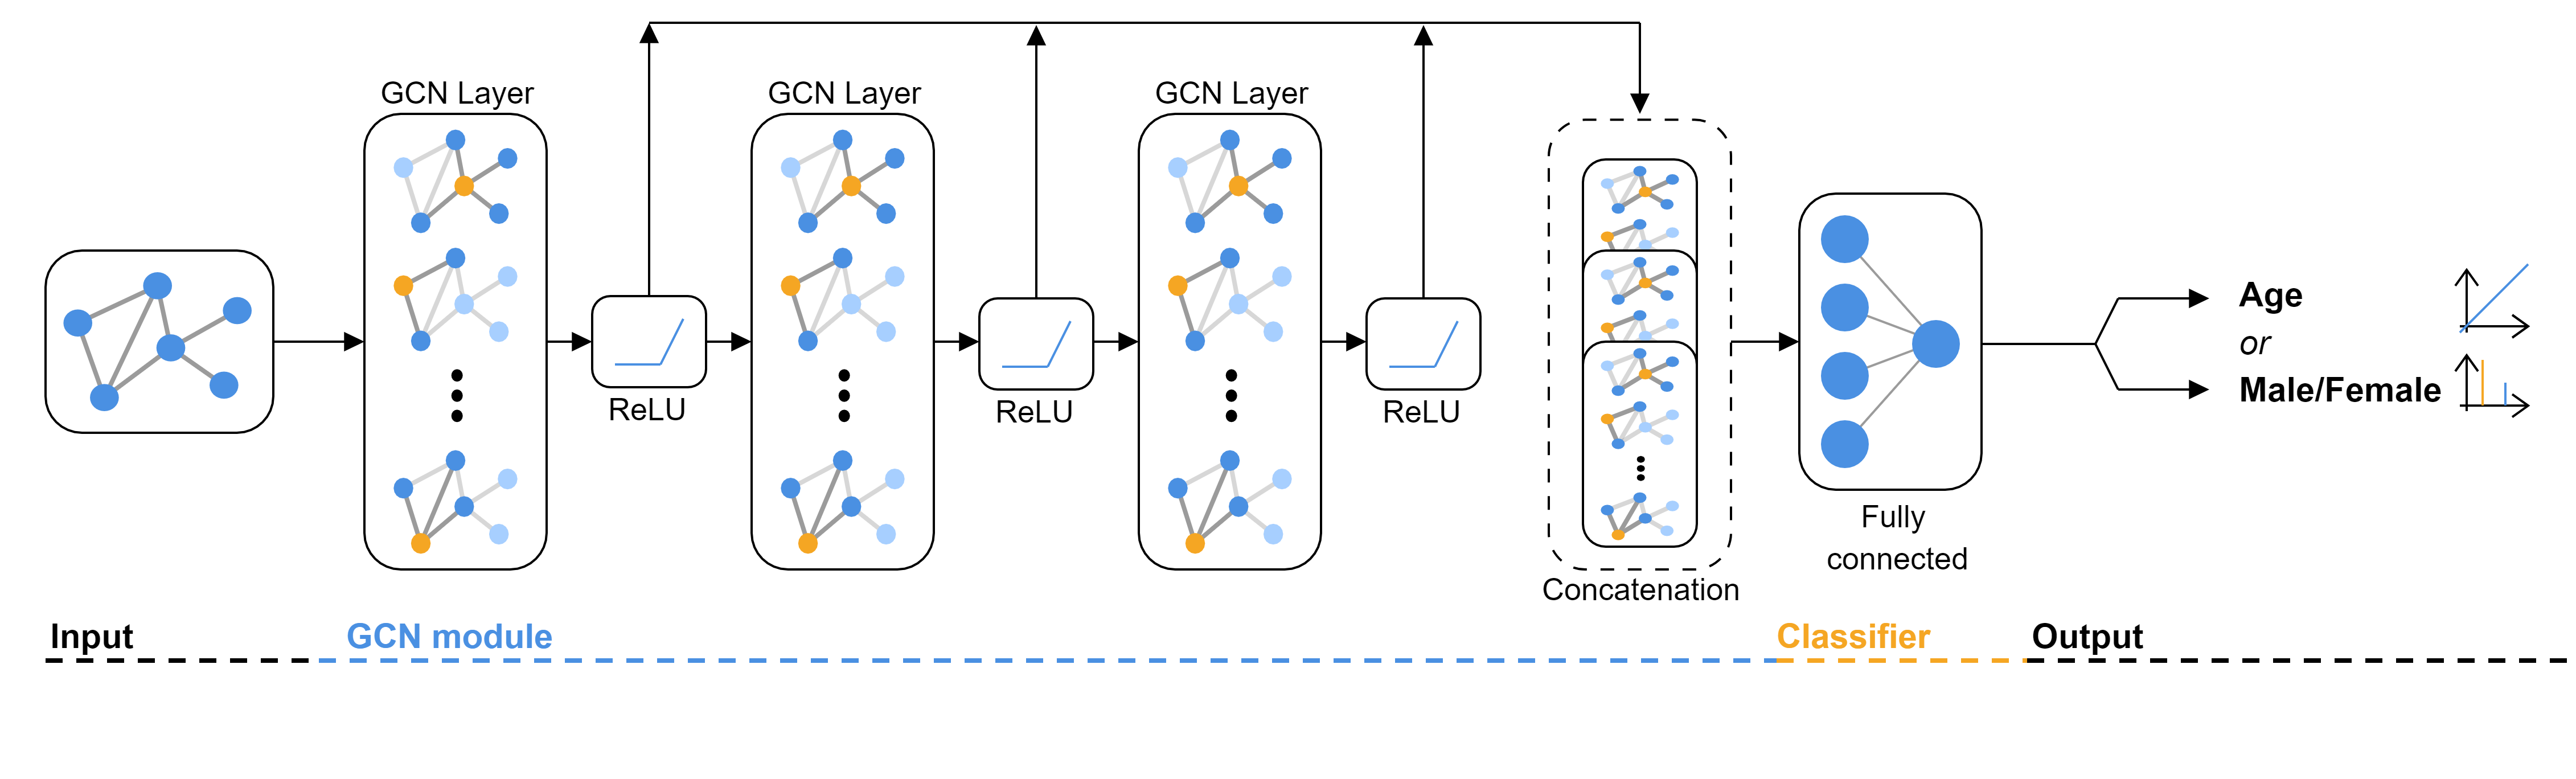
\includegraphics[width=\textwidth]{chapters/images_methods/base_v2.png}
    \caption{The GCN model, which takes a single brain graph as input and outputs a predicted age or sex. The input graph is processed through three graph convolutional layers with ReLU activation, after which the activations for each layer is concatenated together and fed into a fully connected layer.}
    \label{fig:gcn_base}
\end{figure}


\section{Models for node classification}

With the models performing graph predictions introduced, two models used to perform node prediction on a population graph will now be presented. First, however, the procedure of forming population graphs will be described, followed by a batching method that enables models to be trained.

\subsection{Forming population graphs}

As discussed in \cref{sec:similarity_measure}, the design of the similarity measure is an important decision and should be done with the given application in mind. For our specific application, it's desirable that subjects that have similar \acrshort{fmri} data are connected with edges that have large weights, with the idea that the models will be able to draw upon this information of similarity to yield a better inference. A general construction that fulfils this requirement is the use of a distance metric inverted by a kernel, as described in Equation \eqref{eq:similarity_measure}. With this construction, and given two subjects and their adjacency matrices $A_1$ and $A_2$, we defined the similarity measure $\sigma\left(A_1, A_2, l\right)$ as
\begin{equation}
    \sigma\left(A_1, A_2, l\right) = \exp{\left(- \frac{||A_1 - A_2||_F^2}{l||A_1||_F ||A_2||_F} \right)}\biggr\rvert_{l=0.5},
    \label{eq:modified_similarity_measure}
\end{equation}
where $||A_1 - A_2 ||_F$ is the matrix Frobenius norm of the difference between $A_1$ and $A_2$. The Frobenius norm is defined as $||A||_F = \left( \sum_i \sum_j |A_{ij}|^2 \right)^{1/2}$. The norm of the difference was weighted with a hyperparameter $l=0.5$ and the norms of $A_1$ and $A_2$, and then fed into a Gaussian kernel. The Gaussian kernel ensured that larger differences between $A_1$ and $A_2$ yielded smaller similarity scores $\sigma\left(A_1, A_2, l\right)$, and also that  $\sigma\left(A_1, A_2, l\right) \in \left[0, 1\right]$. As desired, subjects that had similar fMRI data, and thus a smaller difference between their adjacency matrices, obtained a larger similarity score and vice versa. 

% Note that the similarity measure in equation \eqref{eq:modified_similarity_measure} only utilises the \acrshort{fmri} data for each subject. One could imagine a similarity measure that uses other types of data that is related to the tasks of predicting age/sex, such as eventual brain-health related diagnosis \cite{stankeviciute}. The choice of only using \acrshort{fmri} data was motivated by two reasons; partly because using other data sources requires extensive domain knowledge, and partly because we are specifically interested in the predictive power of \acrshort{fmri} data, without introducing other confounding variables.

\subsection{Batches of population graphs}
The adjacency matrix for a population graph quickly becomes very large, since the number of edges in the graph grows with the number of subjects squared. For example, a population graph with 30 000 subjects requires approximately 7 GB of memory to store. This is a problem, since predicting and training using such a large matrix is time consuming, and the memory consumption can also be problematic. To resolve this problem, and thus in a feasible way be able to train models on population graphs including all the data, a batching method was developed. 

\begin{figure}[!htbp]
    \centering
    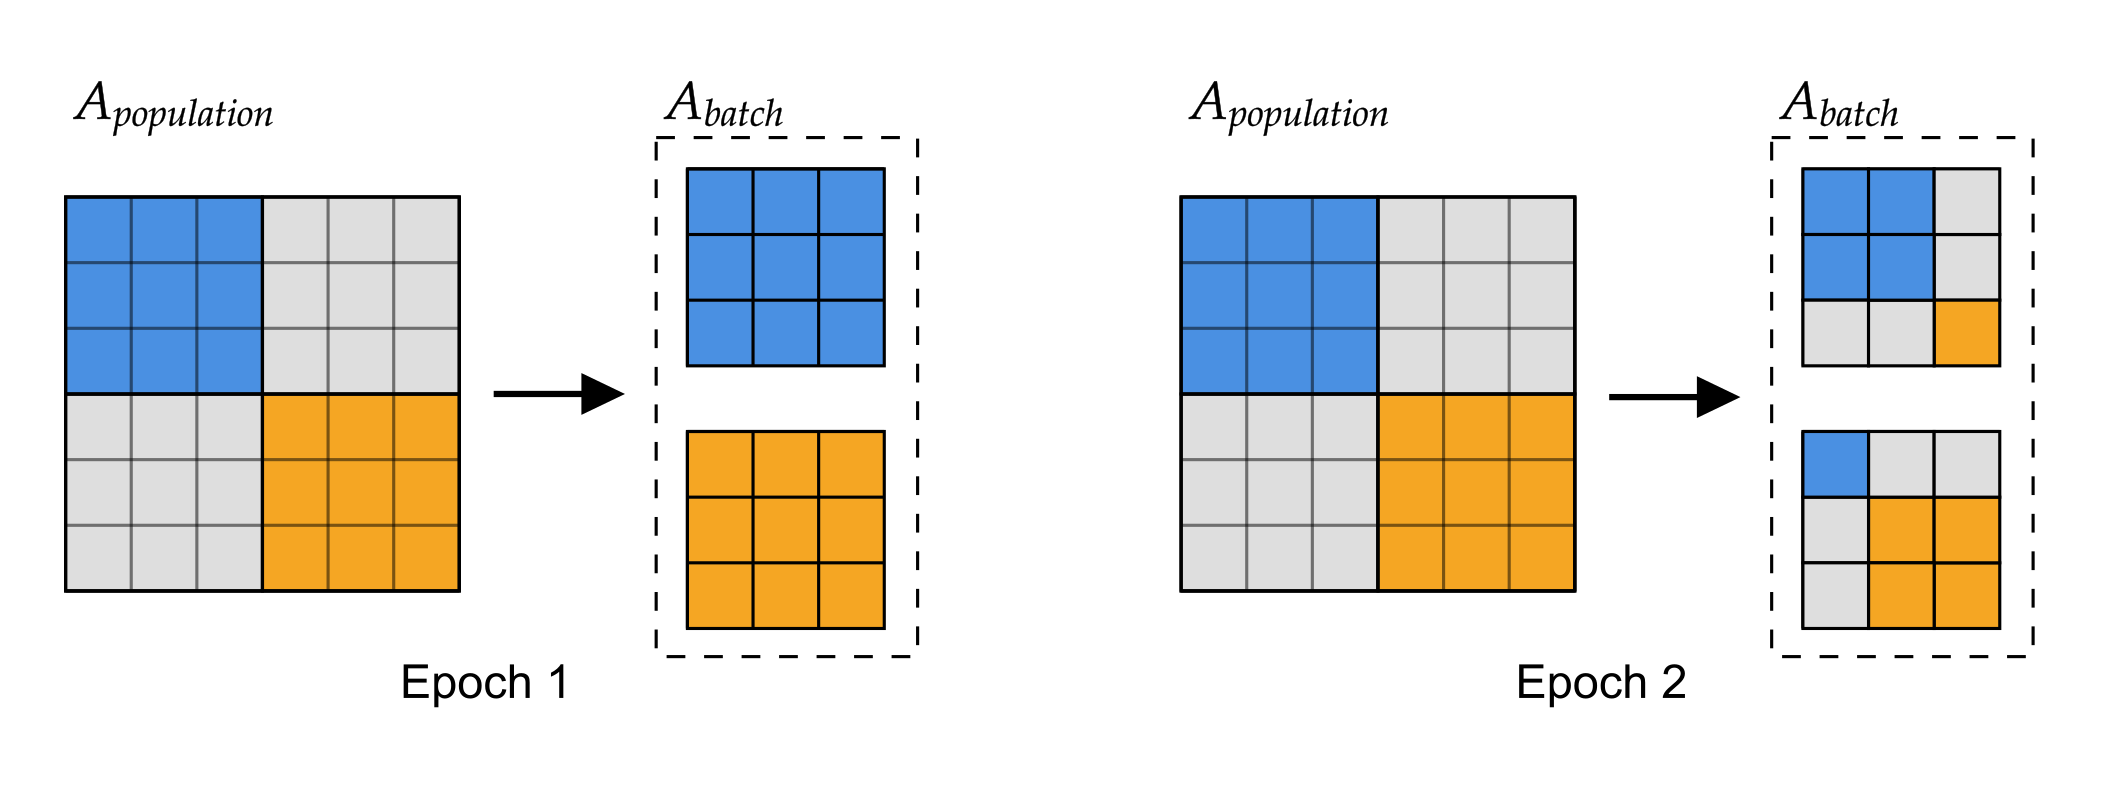
\includegraphics[width=0.9\textwidth]{chapters/images_methods/batching.png}
    \caption{An example of the batching approach for splitting a large population graph $A_{population}$ into two smaller population graphs, each corresponding to a batch $A_{batch}$. In the first epoch, only the connections between the first three (blue) and last three (orange) subjects are included in the batched population graphs. By permuting which subjects are included in each of the smaller population graphs for the second epoch and onwards, all connections not included in the first epoch (gray) will eventually be sampled.}
    \label{fig:batches}
\end{figure}

The batching method was based on dividing the population graph into several smaller population graphs. This was done by splitting the data set into several smaller data sets of 100 subjects each and constructing one population graph for each smaller data set. In practice, this was done by extracting all connections between the 100 subjects from the larger population graph. For an illustration on how this was done see \cref{fig:batches}. With this batching approach, dividing a population graph of 30 000 subjects into for instance 300 smaller graphs with 100 nodes each would require 24 MB of memory, as compared to 7 GB before batching. This is a difference of roughly two orders of magnitude.

As seen in \cref{fig:batches}, many of the connections between subjects are not utilised if the population graph is divided into several smaller graphs. To solve this, the way the subjects were divided into smaller graphs was changed between epochs as seen in \cref{fig:batches}. By always changing which people were combined in the graphs, all connections were eventually used after enough epochs. The advantage of always changing the subjects that were included in the graphs was that the models could not overfit against a specific graph structure. The models were thus forced to learn very general patterns to make predictions for all subjects in the graphs. However, this generalisation might also be a disadvantage, since overfitting on the graph structure may yield higher validation performance as long as the graph structure remains fixed. 

\subsection{Poptoy}

As a first model for predictions on a population graph, the Poptoy model was introduced. The input to Poptoy consisted of a population graph, which was then propagated through five graph convolutional layers.  The output layer of Poptoy was a fully connected layer with one or two softmax output neurons, and the input to the fully connected layer consisted of the activations of all layers and all features for a specific node. 
The fully connected output layer was repeatedly used and a prediction for each node, and thus each subject, was made and the number of weights was kept low as the number of nodes in the population graph grew. An illustration of the Poptoy model can be seen in \cref{fig:poptoy}. Poptoy is similar to GCN, but the output layer differs as Poptoy performs node prediction instead of graph prediction. GCN's output layer took the activations for all layers and all features for all nodes as input. 

\begin{figure}[!htbp]
    \centering
    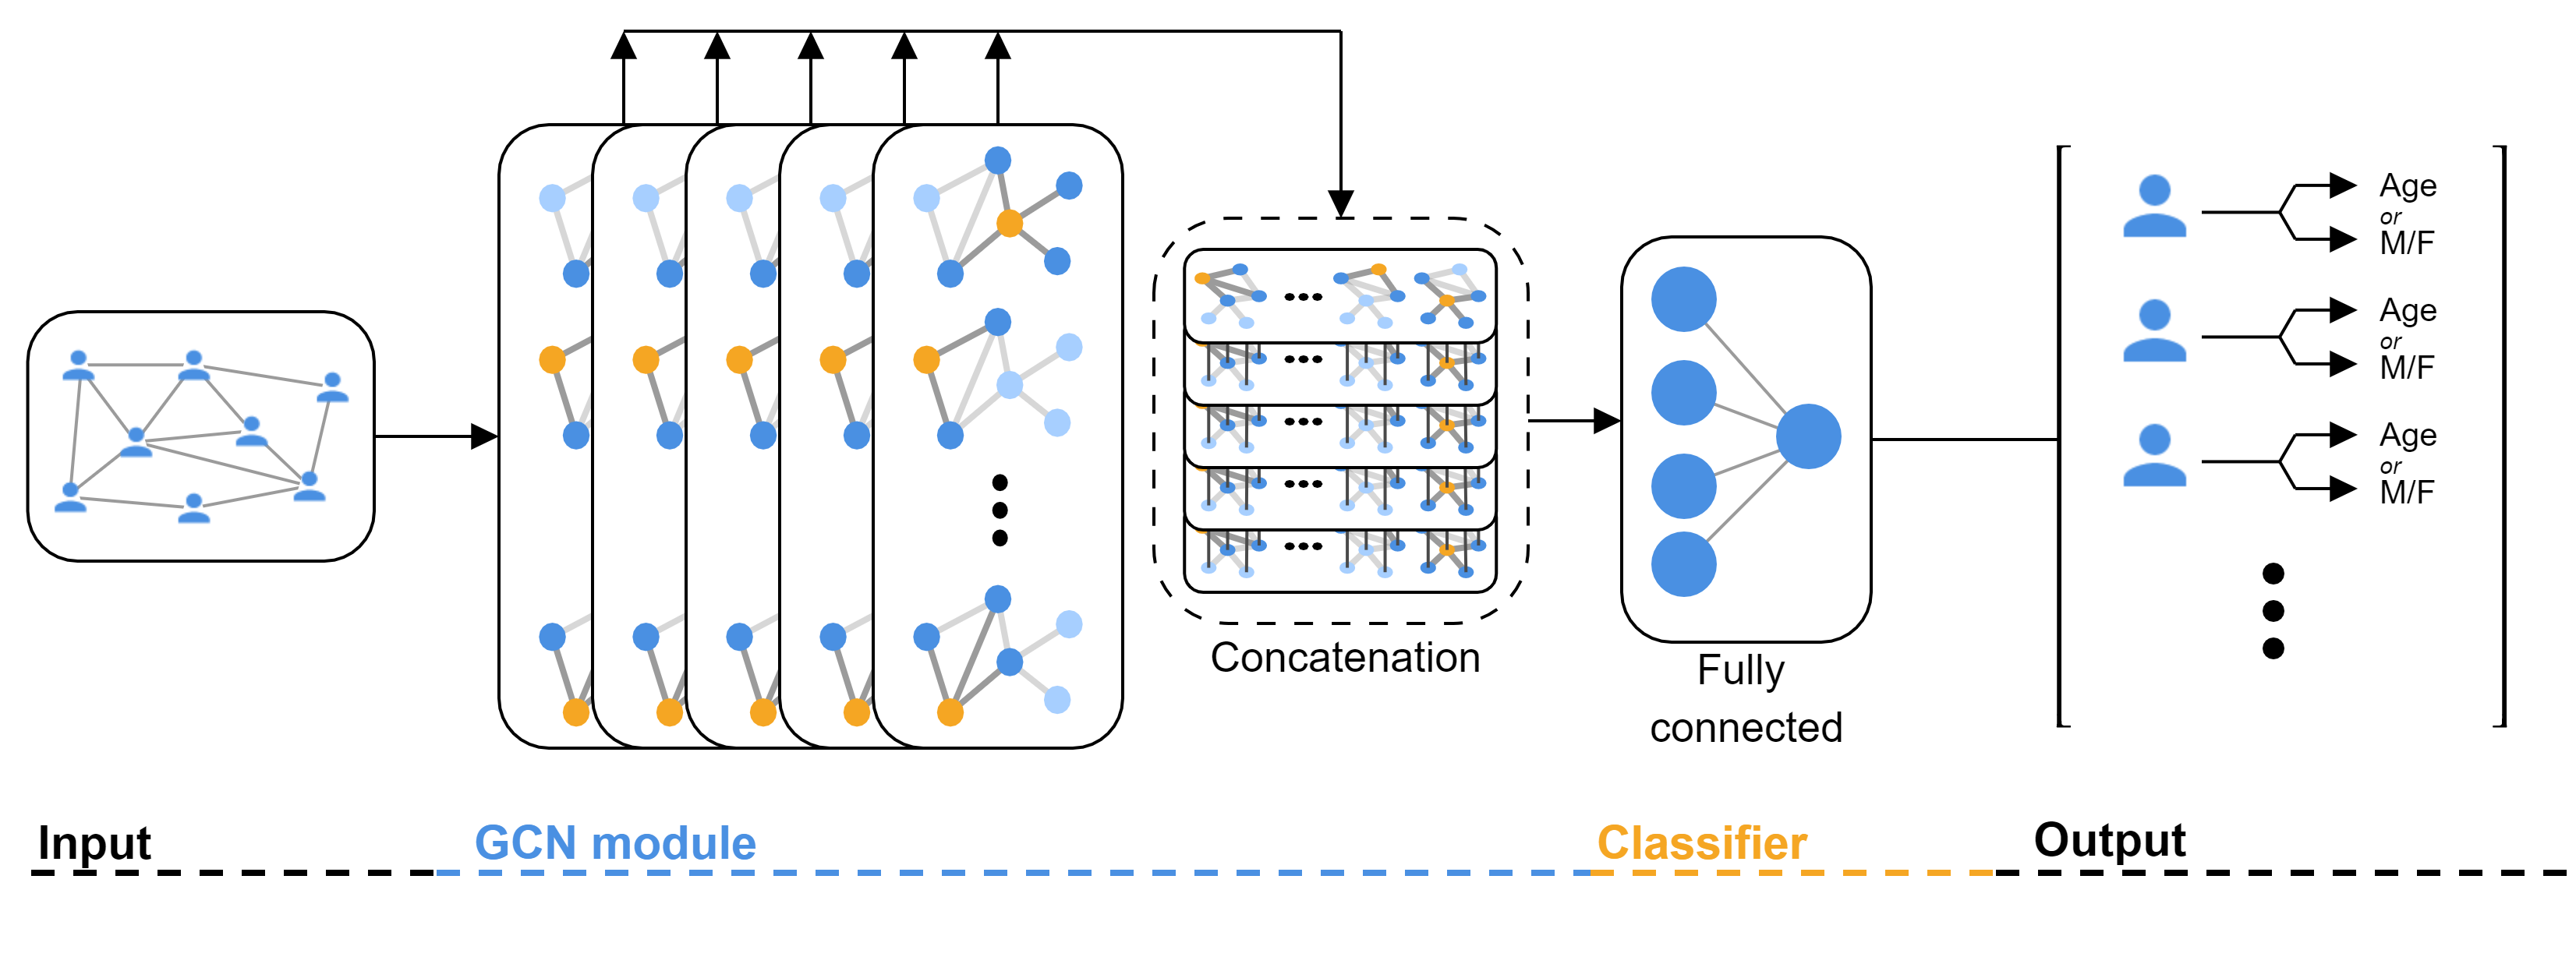
\includegraphics[width=\textwidth]{chapters/images_methods/poptoy_v2.png}
    \caption{The Poptoy model. The input consists of a population graph, which is passed through five graph convolutional layers. The five activations are concatenated together and fed into a fully connected output layer, which outputs a predicted age or sex on a subject-level.}
    \label{fig:poptoy}
\end{figure}

The reason the Poptoy model consisted of five graph convolutional layers instead of three, which GCN had, was that the population graphs became much larger than the individual brain graphs. The individual brain graphs consisted of 21 nodes, which where all more or less connected, and since each graph convolutional layer takes into account one higher order of neighbours, all nodes were to some extent included in the first order neighbourhood. Thus, the need for more graph convolutional layers quickly diminished. For population graphs, the need for considering neighbours further away in the graph might be much larger and hence Poptoy utilised more graph convolutional layers than GCN. Five layers were specifically chosen since adding more layers did not increase performance.

Furthermore, the split into validation and training sets had to be handled, since all subjects in the data set were incorporated in the population graph. To solve this, a set of subjects in the population graph were defined to be the training set, and the rest to be the validation set. The model was then constructed to either do predictions for only the nodes in the training set or validation set. Then, the training could be performed while only doing predictions on the set and vice versa when evaluating. 




\subsection{Popencoder}
As a means to incorporate more information about each subject in the population graph, a model referred to as Popencoder was designed. The Popencoder model is identical to Poptoy in the sense that the population graph was propagated through five graph convolutional layers, after which a prediction for each nodes was made using a fully connected layer. The difference is that in Popencoder, features for each node were introduced. The features were based on the adjacency matrices of each individual subject, but to compress the dimensionallity of the feature space these matrices were encoded into a lower dimensional space. The encoder consisted of two graph convolutional layers followed by a fully connected layer with either two softmax activated neurons or one linearly activated neuron, in the case of sex or age prediction respectively. For an illustration of Popencoder, see \cref{fig:popencoder}.

A heuristic explanation of why the features introduced to the population graph would help, is that the encoder can make an initial prediction of the age or sex for each individual subject. Then, by propagating this information through the population graph, the information of similarities to other subjects in the data set possibly can improve on the predictions. In that case, one could argue that the initial prediction might be done as a preprocessing step, for example via a prediction with another model. The encoding is, however, viewed as a trainable part of the model to allow for more abstract and advantageous embeddings to be learnt during model training. 



\begin{figure}[!htbp]
    \centering
    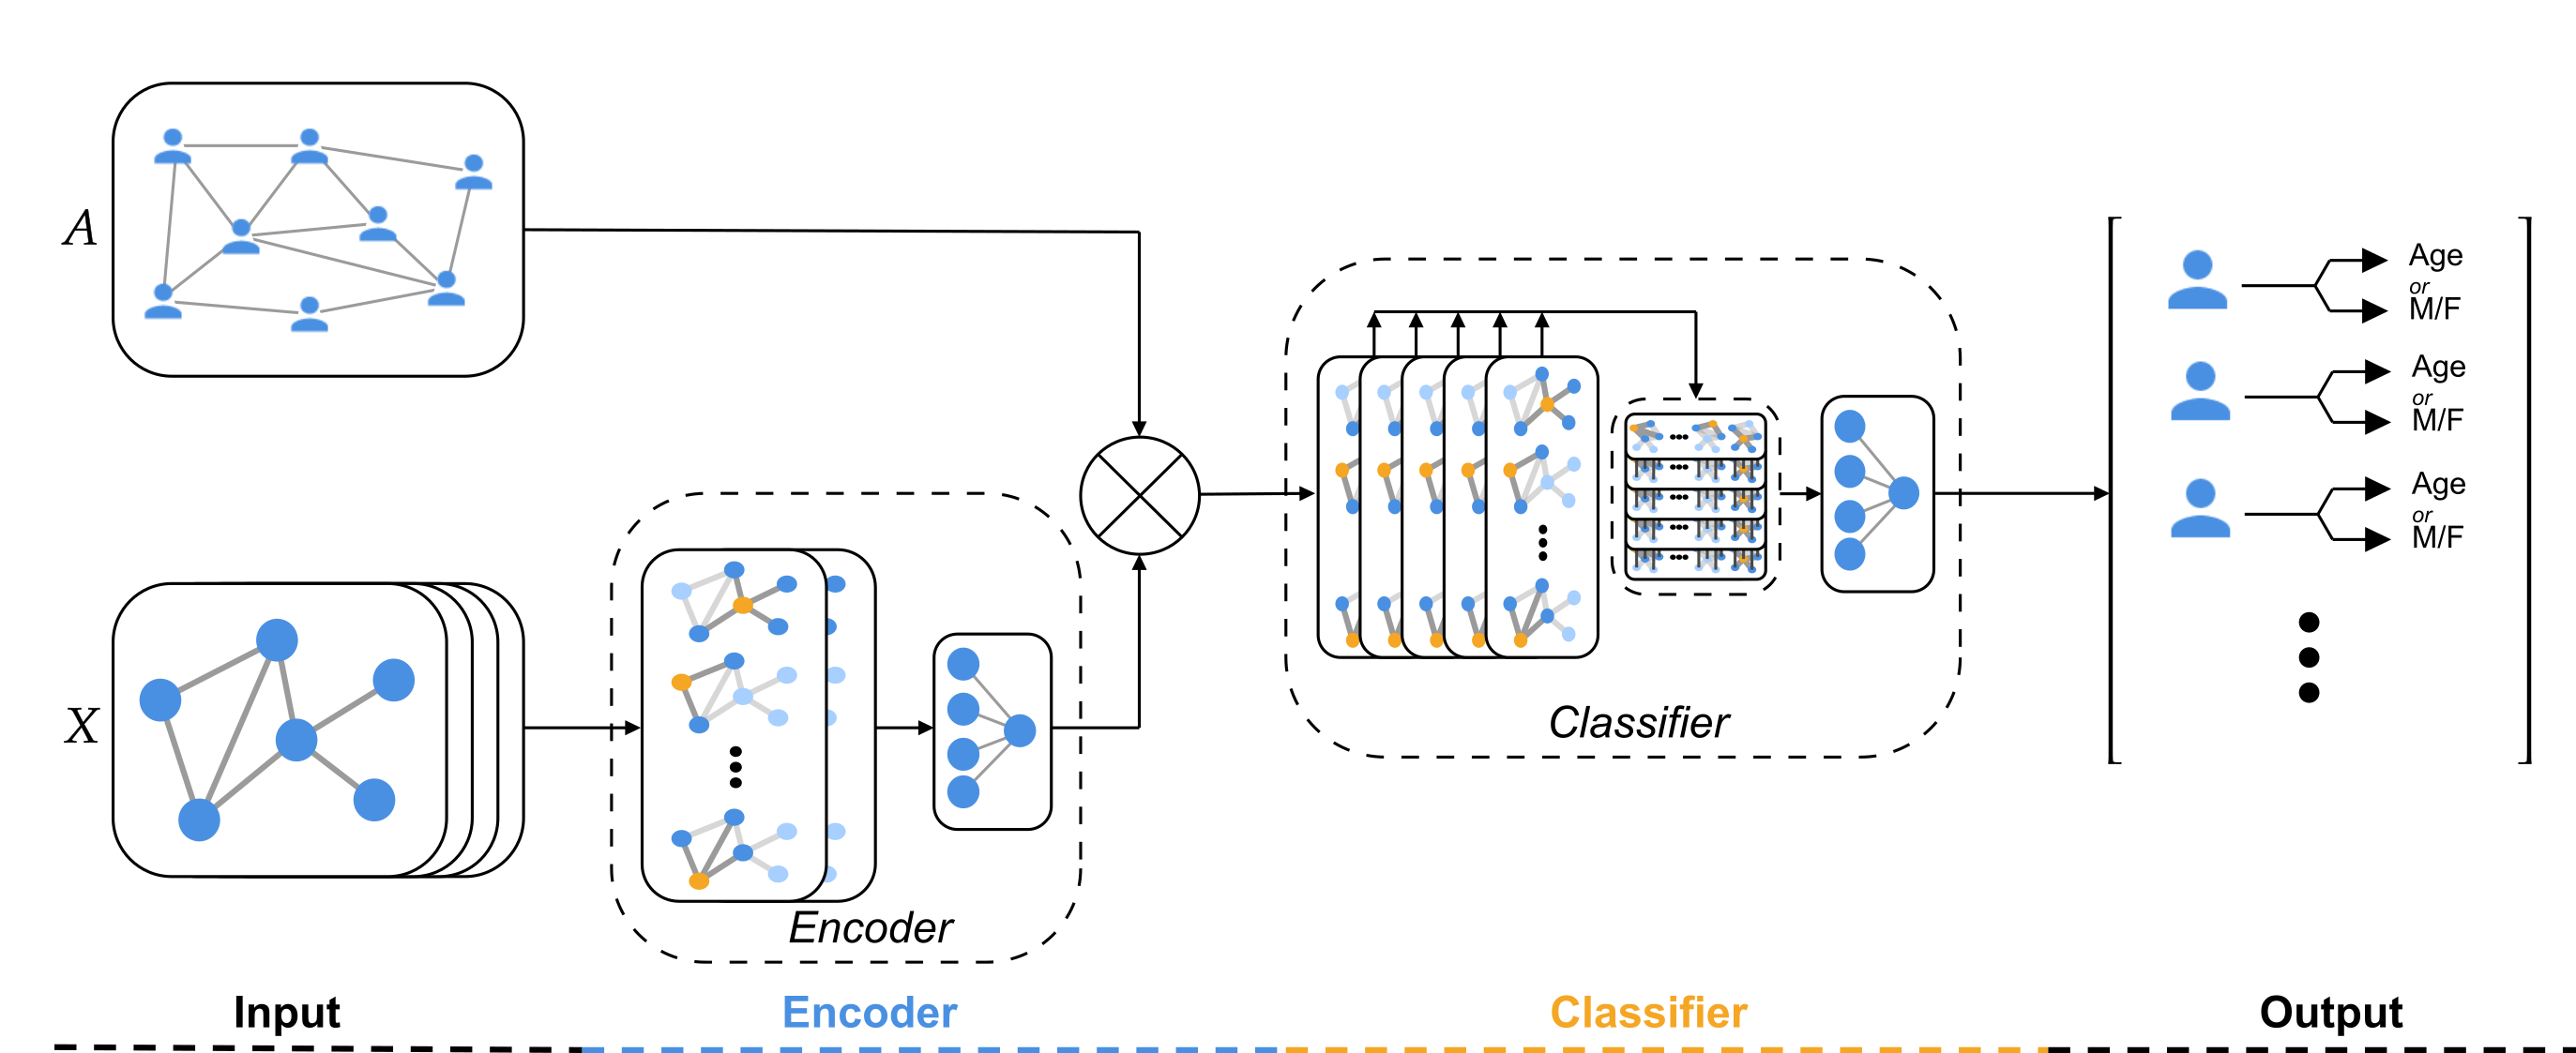
\includegraphics[width=0.9\textwidth]{chapters/images_methods/popencoder_v2.png}
    \caption{The Popencoder model, which takes two inputs: a population graph $A$, and the brain graphs for all subjects in the population graph, $X$. The brain graphs are passed through an encoder, consisting of two graph convolutional layers followed by a fully connected layer. The encoded brain graphs and the population graph $A$ are then fed into the Classifier, which consists of five graph convolutional layers followed by a concatenation and fully connected layer. The output is a predicted age or sex on a subject-level.}
    \label{fig:popencoder}
\end{figure}

\section{Model explainability through saliency mapping}
To determine what functional networks in the brain are related to sex and age, model analysis, in the form of analysing what the models have learned, is an essential part of the work. Specifically, using saliency mapping techniques to analyse which nodes in the brain graph are important for making predictions will by extension give information on what functional networks are important, due to each node representing a functional network. 

Two methods for model analysis was used: a naive approach based on node removal, and a more sophisticated method for node masking based on the Zorro algorithm described in \cref{sec:zorro}. Note that these are not methods that open up the black-box of neural networks per say (by e.g. parameter analysis). These methods analyse/explain the networks from an outer perspective, which is beneficial as it poses no assumption on the model architecture, only in- and output data. Thus, the same analysis may be performed for different models, making it also beneficial for validation and result comparison. 

\subsection{Naive node removal}
A simple method to obtain a saliency map of which nodes are important for predictions is a node removal method. This particular method is self-composed, and consisted of simply removing a specific node for every subject in the data set, after which a new model was retrained. By comparing the predictive performance of the retrained model with a reference model trained on data with no nodes removed, an indication of the importance of that node could be obtained. This is based on the assumption that a large loss in performance means vital information for the prediction had been removed, which was interpreted to be indicative of the importance of that node. The method was then be repeated for all nodes in order to obtain a measure of importance for each node.


\subsection{Zorro}

The Zorro algorithm, described in \cref{sec:zorro}, was developed for saliency mapping of models with graph features as input. It thus needed to be modified to be applied to the models presented in this thesis. The need for modification arose since our Baseline and GCN models are completely featureless approaches that only takes an adjacency matrix $A$ as input. Therefore, it was not possible to introduce noise to the feature matrix, as done in the original method. Instead, it had to be done on $A$. The reintroduction of nodes in $A$, in the following referred to as unmasking, could have been done in two ways; either on a connection level where entries in $A$ are unmasked, or on a nodal level where whole rows and columns in $A$ are unmasked. We were primarily interested in which nodes were important, so the latter was used. Unmasking whole nodes instead of connections also yielded computational benefits, since the number of nodes was less than the number of connections. As whole nodes were unmasked, the explanation in the modified Zorro method only contained a set of nodes, $\mathcal{S} = \{V\}$. The masked adjacency matrix was then given by 
\begin{equation*}
    B_S = A \odot S + Z \odot (1- S), \quad Z \sim \mathcal{N},
\end{equation*}
where $S$ is the masking matrix for the explanation $\mathcal{S}$, and the model predictions are $\Phi(A)$ and $\Phi(B_S)$. For age prediction, $\Phi(B_S)$ was deemed correct if $\left|\Phi(A) - \Phi(B_S)\right| < t$ for some tolerance $t$, since age is a continuous variable. The noise $Z$ was drawn from a Gaussian distribution with mean and standard deviation given by the entries of $A$ over the data set. The fidelity was calculated in the same way as in the original algorithm, and an explanation $\mathcal{S}$ for an individual subject was still accepted if the fidelity of $\mathcal{S}$ was higher than $\tau$. 

Lastly, since the algorithm yielded which nodes were important for the prediction of an individual subject, the procedure was repeated for several subjects to get a sense of which nodes are generally important. To evaluate the importance of each node, an importance score $\mathcal{I}$ was introduced as the number of explanations $\mathcal{S}$ a node was included in, divided by the total number of subjects. An importance score of $\mathcal{I}=1$ indicates that the node is considered important for the prediction of all subjects, and a score of $\mathcal{I}=0$ for none.  